\documentclass{article}

% if you need to pass options to natbib, use, e.g.:
%     \PassOptionsToPackage{numbers, compress}{natbib}
% before loading neurips_2025

% The authors should use one of these tracks.
% Before accepting by the NeurIPS conference, select one of the options below.
% 0. "default" for submission

\PassOptionsToPackage{round,authoryear}{natbib}
 % \usepackage{neurips_2026}
 \usepackage[preprint]{neurips_2025}
% the "default" option is equal to the "main" option, which is used for the Main Track with double-blind reviewing.
% 1. "main" option is used for the Main Track
 % \usepackage[main]{neurips_2025}
% 2. "position" option is used for the Position Paper Track
%  \usepackage[position]{neurips_2025}
% 3. "dandb" option is used for the Datasets & Benchmarks Track
 % \usepackage[dandb]{neurips_2025}
% 4. "creativeai" option is used for the Creative AI Track
%  \usepackage[creativeai]{neurips_2025}
% 5. "sglblindworkshop" option is used for the Workshop with single-blind reviewing
 % \usepackage[sglblindworkshop]{neurips_2025}
% 6. "dblblindworkshop" option is used for the Workshop with double-blind reviewing
 % \usepackage[dblblindworkshop]{neurips_2025}

% After being accepted, the authors should add "final" behind the track to compile a camera-ready version.
% 1. Main Track
 % \usepackage[main, final]{neurips_2025}
% 2. Position Paper Track
%  \usepackage[position, final]{neurips_2025}
% 3. Datasets & Benchmarks Track
 % \usepackage[dandb, final]{neurips_2025}
% 4. Creative AI Track
%  \usepackage[creativeai, final]{neurips_2025}
% 5. Workshop with single-blind reviewing
%  \usepackage[sglblindworkshop, final]{neurips_2025}
% 6. Workshop with double-blind reviewing
%  \usepackage[dblblindworkshop, final]{neurips_2025}
% Note. For the workshop paper template, both \title{} and \workshoptitle{} are required, with the former indicating the paper title shown in the title and the latter indicating the workshop title displayed in the footnote.
% For workshops (5., 6.), the authors should add the name of the workshop, "\workshoptitle" command is used to set the workshop title.
% \workshoptitle{WORKSHOP TITLE}

% "preprint" option is used for arXiv or other preprint submissions
 % \usepackage[preprint]{neurips_2025}

% to avoid loading the natbib package, add option nonatbib:
%    \usepackage[nonatbib]{neurips_2025}

\usepackage[utf8]{inputenc} % allow utf-8 input
\usepackage[T1]{fontenc}    % use 8-bit T1 fonts
\usepackage{hyperref}       % hyperlinks
\usepackage{url}            % simple URL typesetting
\usepackage{booktabs}       % professional-quality tables
\usepackage{amsfonts}       % blackboard math symbols
\usepackage{nicefrac}       % compact symbols for 1/2, etc.
\usepackage{microtype}      % microtypography
\usepackage{xcolor}         % colors
\usepackage{xspace}

\usepackage[most]{tcolorbox}
\usepackage[table]{xcolor}

\usepackage[export]{adjustbox}

\usepackage{amssymb}
\usepackage{mathtools}

\usepackage{subcaption}
\usepackage{graphicx}
\usepackage{etoolbox}

\usepackage{wrapfig}

\usepackage{booktabs}
\usepackage{multirow}
\usepackage{amsmath}
\usepackage{makecell}

\usepackage{algorithm}
\usepackage{algorithmic}

% --- code boxes ---
\usepackage[most]{tcolorbox}
\usepackage{listings}
\usepackage{xcolor}

\definecolor{boxbg}{gray}{0.96}
\definecolor{boxframe}{gray}{0.35}

\lstdefinestyle{mytt}{
  basicstyle=\ttfamily\footnotesize,
  columns=fullflexible,
  breaklines=true,
  showstringspaces=false,
  numbers=left,
  numberstyle=\tiny\color{gray},
  numbersep=6pt,
  xleftmargin=1.2em,
  frame=none
}

% 一个可换页、圆角、灰底的“框环境”
\newtcolorbox{promptbox}[1][]{
  enhanced,
  breakable,              % 允许跨页
  colback=boxbg,
  colframe=boxframe,
  boxrule=0.8pt,
  arc=2mm,                % 圆角
  left=2mm,right=2mm,top=1.5mm,bottom=1.5mm,
  #1
}


\definecolor{envbg}{RGB}{255, 247, 237}   % 很浅橙（背景）
\definecolor{envframe}{RGB}{230, 140, 60} % 柔和橙（边框）
\newtcolorbox{envbox}[1][]{
  enhanced,
  breakable,              % 允许跨页
  colback=envbg,
  colframe=envframe,
  boxrule=0.8pt,
  arc=2mm,                % 圆角
  left=2mm,right=2mm,top=1.5mm,bottom=1.5mm,
  #1
}

\definecolor{herabg}{RGB}{240, 247, 255}
\definecolor{heraframe}{RGB}{100, 150, 220}
\newtcolorbox{herabox}[1][]{
  enhanced,
  breakable,              % 允许跨页
  colback=herabg,
  colframe=heraframe,
  boxrule=0.8pt,
  arc=2mm,                % 圆角
  left=2mm,right=2mm,top=1.5mm,bottom=1.5mm,
  #1
}

% ===== 方案3：浅绿色（适合 method / algorithm）
\definecolor{devicebg}{RGB}{240, 252, 245}   % 很浅绿（背景）
\definecolor{deviceframe}{RGB}{110, 170, 140} % 柔和绿（边框）
\newtcolorbox{devicebox}[1][]{
  enhanced,
  breakable,
  colback=devicebg,
  colframe=deviceframe,
  boxrule=0.8pt,
  arc=2mm,
  left=2mm,right=2mm,top=1.5mm,bottom=1.5mm,
  #1
}

% ===== 方案4：浅紫色（适合 theory / analysis）
\definecolor{cloudbg}{RGB}{248, 245, 255}    % 很浅紫（背景）
\definecolor{cloudframe}{RGB}{150, 130, 200} % 柔和紫（边框）
\newtcolorbox{cloudbox}[1][]{
  enhanced,
  breakable,
  colback=cloudbg,
  colframe=cloudframe,
  boxrule=0.8pt,
  arc=2mm,
  left=2mm,right=2mm,top=1.5mm,bottom=1.5mm,
  #1
}

\ifodd 1
\definecolor{darkgreen}{RGB}{0,200,0}
\newcommand{\rev}[1]{{\color{blue}#1}} %revise of the text
\newcommand{\newrev}[1]{{\color{red}#1}} %revise of the text
\newcommand{\needrev}[1]{{\color{darkgreen}#1}} %revise of the text
\else
\newcommand{\rev}[1]{#1}
\newcommand{\newrev}[1]{#1} %revise of the text
\newcommand{\needrev}[1]{#1} %revise of the text
\fi

\newcommand{\name}{Hera\xspace} 

% Note. For the workshop paper template, both \title{} and \workshoptitle{} are required, with the former indicating the paper title shown in the title and the latter indicating the workshop title displayed in the footnote. 
\title{\raisebox{-0.2\height}{
\includegraphics[height=1.2em]{figures/logo.png}}\xspace \name: Learning Long-Horizon Coordination for Device--Cloud Collaborative LLM Agents}


% The \author macro works with any number of authors. There are two commands
% used to separate the names and addresses of multiple authors: \And and \AND.
%
% Using \And between authors leaves it to LaTeX to determine where to break the
% lines. Using \AND forces a line break at that point. So, if LaTeX puts 3 of 4
% authors names on the first line, and the last on the second line, try using
% \AND instead of \And before the third author name.


\author{
Yuxin Zhang$^{1,2}$ \\ \And
Mengxue Hu$^{1}$ \\ \And
Zheng Lin$^{3}$ \\ \And
Xiaoyi Fan$^{4}$ \\ \And
Fan Xie$^{5}$ \\ \And
Zihan Fang$^{1}$ \\ \And
Jing Yang$^{6}$ \\ \And
Wenjun Zhu$^{1,7}$ \\ \And
Zhiwen Chen$^{2}$ \\ \And
Chengfei Lv$^{2}$ \\ \And
Zhe Chen$^{1,7,*}$\\ \And
\texttt{$^{1}$Fudan University \quad
$^{2}$Alibaba Group \quad $^{3}$The University of Hong Kong}\\
\texttt{$^{4}$Shenzhen MSU-BIT University \quad  $^{5}$New York University \quad $^{6}$Universiti Malaya} \\\texttt{$^{7}$SpaceAIC Co., Ltd.}
}

% \author{
%   Haotian Zhao$^1$\thanks{Equal contribution.} \\
%   \And
%   Yuxin Zhang$^1$\footnotemark[1] \\
%   \And
%   Songlin Zhou$^2$\footnotemark[1] \\
%   \AND
%   Stephen S.-T. Yau$^3$\\
%   \And
%   Wenyu Zhang$^1$ \\
%   \And
%   Tianshu Zhu$^1$ \\
%   \And
%   Lun Tian$^1$ \\
%   \And
%   Yucheng Zeng$^1$ \\
%   \And
%   Yifeng Huang$^4$ \\
%   \And
%   Jingnan Gu$^1$\thanks{Corresponding author.} \\
%   \And
%   Daxiang Dong$^1$\footnotemark[2] \\
%   \And
%   Jianmin Wu$^1$\footnotemark[2] \\
%   \AND
%   $^1$\texttt{\{zhaohaotian02,zhangyuxin15,zhangwenyu08,zhutianshu,tianlun,}\\
% \texttt{zengyucheng,gujingnan,dongdaxiang,wujianmin\}@baidu.com}, \quad Baidu\\
%   $^2$\texttt{zhousl24@mails.tsinghua.edu.cn},\quad Tsinghua University\\
%   $^3$\texttt{yau@uic.edu}, \quad Tsinghua University\\
% %$^4$\texttt{yucheng-zeng@outlook.com},\quad Baidu\\
%   $^4$\texttt{yfhuang24@m.fudan.edu.cn},\quad Fudan University
% }

\begin{document}

\maketitle

\begin{abstract}
% Large language model (LLM) agents integrate language understanding, environmental interaction, and long-horizon decision-making, achieving remarkable success in autonomously solving complex tasks.
% Current device--cloud LLM routers are tailored to static, task-level inference, and ill-suited to agent settings with multi-turn interactions and continuously evolving environments.
% Large language model (LLM) agents have shown strong capability in autonomously interacting with environments to solve complex, long-horizon tasks.
% However, deploying them in real-world settings poses a \textit{device--cloud dilemma}:
Large language model (LLM) agents excel at solving complex long-horizon tasks through autonomous interaction with environments. However, their real-world deployment faces a fundamental \textit{device--cloud dilemma}: 
on-device models are efficient but often brittle, while cloud models are stronger but costly in computation. State-of-the-art LLM device--cloud routers usually make coarse task-level decisions, which cannot adapt to the changing difficulty of multi-step agent interactions.
% small on-device models offer efficiency but lack robustness, while cloud-based large models provide superior capability at prohibitive computational costs.
% State-of-the-art device–cloud LLM routers operate only at the task-level, failing to provide the fine-grained, step-wise coordination required for dynamically evolving, multi-step agent interactions.
% Existing device–cloud LLM routers typically make coarse, task-level decisions, failing to provide fine-grained coordination for agents operating over multi-step interactions in dynamically evolving environments.
% To bridge this gap, we present \name, a \textit{step-level} device--cloud agent coordinator for long-horizon tasks that selectively invokes the cloud at critical states, thereby achieving an optimal performance--cost trade-off.
To address this issue, we present \name, a \textit{step-level} device--cloud LLM agent coordinator for long-horizon tasks achieving a strong performance--cost Pareto frontier.
\name adopts a novel two-stage training paradigm: (1) imitation learning for cold-start, followed by (2) reinforcement learning that jointly optimizes task success and cloud usage efficiency.
% reinforcement learning that maximizes task success while minimizing cloud usage.
The first stage casts step-level routing as a supervised classification problem: the device agent is replayed on cloud trajectories, with each state labeled by the agreement between device and cloud actions.
In the second stage, we perform cost-aware reinforcement learning by grouping identical states across trajectories and updating \name with labels favoring higher expected return and fewer future cloud calls.
We evaluate \name on ALFWorld, WebShop, and AppWorld, where it consistently outperforms prior methods,
achieving 92.5\% of the cloud-only success rate with cloud use in only 46.3\% of steps.
% using cloud calls in only \needrev{xx\%} steps while surpassing a cloud-only model by \needrev{xx\%} in success rate.
% We evaluate \name on ALFWorld, WebShop, and AppWorld benchmarks, where it consistently outperforms existing methods, achieving the highest task success with the lowest cloud usage.
\end{abstract}

% However, their real-world deployment faces a \textit{device--cloud dilemma}: user-end models provide low latency and cost but limited performance, while cloud-based models offer superior intelligence at the expense of high latency and substantial expense.
% To bridge this gap, we present \name, a \textit{step-level} device–cloud agent coordinator that detects critical states in long-horizon tasks and selectively invokes the cloud, thereby achieving an optimal performance--cost trade-off.

% Recent advances in large language models (LLMs)~\citep{singh2025openai,yang2025qwen3,liu2024deepseek}, particularly in long-horizon reasoning and interactive decision-making, combined with agentic frameworks such as ReAct~\citep{Yao2023ReAct}, have enabled LLM agents to perform complex, multi-step tasks well beyond static problem solving~\citep{chang2024agentboard}.
% These agents interact with open-ended environments in multi-step cycles, using feedback from each step to inform subsequent actions, and have demonstrated success across diverse domains including software engineering~\citep{zhang2024codeagent,yang2025kimi}, GUI navigation~\citep{vattikondatrain,gurreal}, and interactive gameplay~\citep{wangvoyager,tan2025lumine}, and robotic control~\citep{zitkovich2023rt,hanrobocerebra}.

\section{Introduction}
Recent advances in large language models (LLMs)~\citep{singh2025openai,yang2025qwen3,liu2024deepseek}, combined with agentic frameworks such as ReAct~\citep{Yao2023ReAct}, have empowered LLM agents to perform complex, long-horizon reasoning and decision-making well beyond static problem solving~\citep{chang2024agentboard}.
These agents operate in open-ended environments through multi-step interaction loops, using step-wise feedback to guide subsequent actions, and have demonstrated strong performance across diverse domains, including software engineering~\citep{zhang2024codeagent,yang2025kimi}, GUI navigation~\citep{vattikondatrain,gurreal}, interactive gameplay~\citep{wangvoyager,tan2025lumine}, and robotic control~\citep{zitkovich2023rt,hanrobocerebra}.

Despite their promise, LLM agents in real-world environments face a fundamental device--cloud trade-off.
On one hand, deploying advanced agents directly on user-end is infeasible due to stringent resource constraints.
Small models (e.g., $<$10B parameters) that fit within device memory limits typically exhibit significant performance degradation in complex reasoning tasks, often failing to maintain long-term coherence in multi-step trajectory planning~\citep{nozaki2025efficient,ong2025routellm}. On the other hand, reliance on powerful cloud-based closed-source models introduces substantial network latency and high usage cost, limiting their practicality for real-time applications such as robotic manipulation and interactive GUI navigation~\citep{ravichandran2025distilling,wanyanlook}.
For example, a cloud-based drone navigation agent may miss dynamic obstacles due to network jitter, whereas an on-device model may lack the “System 2” reasoning depth to plan an optimal global path.

To balance local efficiency and global performance, recent work dynamically allocates inference between device- and cloud-side LLMs~\citep{narayan2025cost,li2025collaborative}.
Existing methods treat each request as an atomic unit, making a one-shot routing decision before inference begins by assigning the entire query to a single model based on estimated difficulty, confidence, or preference~\citep{ong2025routellm,Eagle2024}. While effective for standalone tasks such as question answering, summarization, and code completion, this paradigm is poorly suited to long-horizon agent settings, where execution unfolds as a sequence of interdependent steps whose difficulty changes with the evolving environment state~\citep{fenggroup,dong2026agentic}.

% \needrev{Hence, these limitations raise a core question:}

% \begin{tcolorbox}[
%     colback=gray!15,      % 背景灰色
%     colframe=black,       % 边框颜色
%     boxrule=0.8pt,        % 边框粗细
%     arc=3pt,              % 圆角大小
%     left=6pt,
%     right=6pt,
%     top=6pt,
%     bottom=6pt
% ]
% \textit{Can we design a general edge–cloud LLM agent coordinator that achieves optimal performance with minimal cloud reliance through precise step-level routing?}
% \end{tcolorbox}


\begin{figure*}[t]
    \centering
    \vspace{-1.0em}  % 适当调整与标题间距
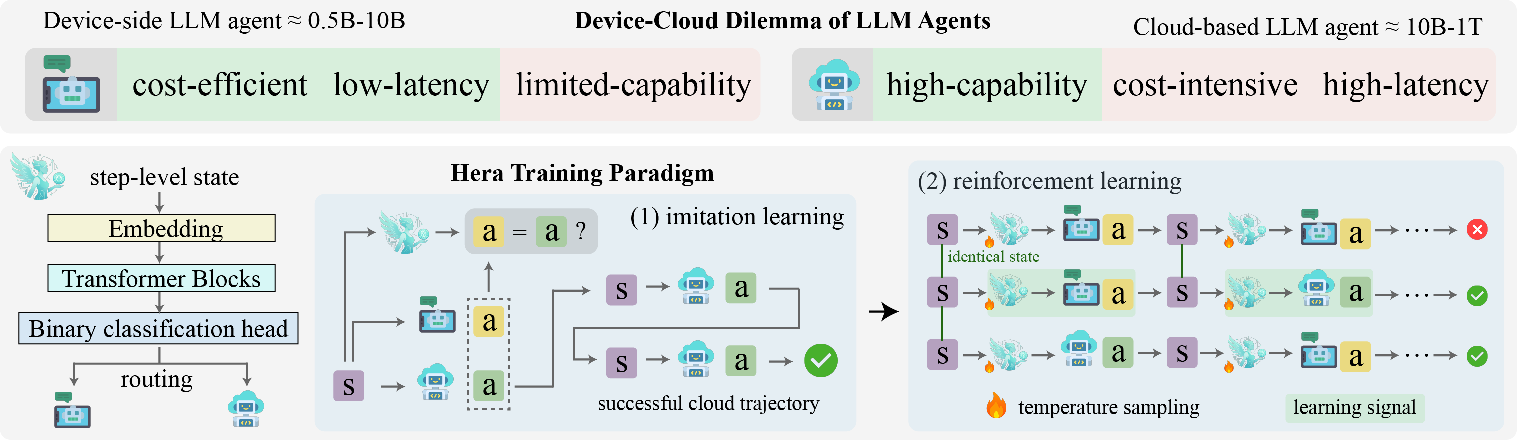
\includegraphics[width=\textwidth,height=8.9cm,keepaspectratio]{figures/teaser.pdf}
\caption{LLM agents face a fundamental device--cloud dilemma. To address this, \name is proposed as a lightweight step-level device--cloud coordinator trained via a two-stage paradigm: imitation learning for cold-start, followed by reinforcement learning for performance--cost co-optimization.}
    \vspace{-1.5em}  % 控制与正文间距
\label{figure:teaser}
\end{figure*}

To address this limitation, this paper investigates \textit{step-level} device--cloud routing for long-horizon LLM agent tasks, aiming to better balance task success and inference cost through routing decisions made at each environment interaction rather than once per task. Importantly, we find that offloading only a small fraction of critical steps along the trajectory to the cloud is sufficient to match the task success of cloud-only execution (\S\ref{sec:motivation}).
Building on this insight, we propose \name, a lightweight yet powerful device--cloud coordinator that identifies when cloud assistance is necessary, reducing cloud usage while maintaining strong task completion.
% Building on this insight, we present \name, a lightweight yet powerful device-cloud LLM agent coordinator that accurately identifies steps that require cloud assistance, thus minimizing cloud usage while maximizing task performance.
\name follows a two-stage training paradigm, as shown in Figure~\ref{figure:teaser}: (1) imitation learning for routing cold-start (\S\ref{sec:hera_il}), and (2) reinforcement learning for cost-performance co-optimization (\S\ref{sec:hera_rl}).
We initialize \name via imitation learning by replaying the device agent on cloud trajectories and labeling each step by device--cloud action consistency.
We then refine \name with cost-aware reinforcement learning: across multiple rollouts, we group identical states and assign step-level preference labels that prioritize higher estimated return and lower expected future cloud usage.
Across various challenging agent benchmarks including ALFWorld~\citep{ALFWorld20}, WebShop~\citep{yao2022webshop}, and AppWorld~\citep{appworld}, \name consistently outperforms existing methods, demonstrating superior success--cost co-optimization.

Our contributions are threefold:
\begin{itemize}
    \item To the best of out knowledge, \name is the first step-level device--cloud agent coordinator, addressing the performance--cost trade-off of deploying LLM agents in long-horizon tasks.
    \item We develop a two-stage training framework for \name: an imitation-learning stage that initializes routing from device--cloud action agreement, followed by a state-grouped reinforcement learning stage that jointly optimizes trajectory return and cloud cost.
    \item Experiments on various agent benchmarks show that \name outperforms state-of-the-art methods, achieving a stronger trade-off between task success and cloud usage.
\end{itemize}

\section{Related work}
\label{subsec::related_work}

\paragraph{LLMs agents.}
Through carefully designed prompting~\citep{Yao2023ReAct,shinn2023reflexion}, enhanced memory and retrieval mechanisms~\citep{wang2024mobile,xu2025amem}, and integration with external tools~\citep{schick2023toolformer,xie2024osworld}, LM agents are capable of executing complex, multi-step tasks that were previously beyond reach~\citep{chang2024agentboard,xie2024travelplanner,wangvagen}.
Recent work uses supervised fine-tuning~\citep{xia2025sand,zhang2024you,li2026reasoning} and, in particular, reinforcement learning~\citep{fenggroup,mai2025agentic,zhang2026land} to enable LLM agents to learn directly from environment interactions rather than static prompts or handcrafted workflows, significantly enhancing long-horizon reasoning and multi-step decision-making and forming a promising paradigm for general-purpose autonomous intelligence~\citep{comanici2025gemini,qwen3.5,liu2025deepseek}.
However, LLM agents face a fundamental device--cloud dilemma: user-end devices are constrained in memory and energy, limiting LLM scale and performance, while offloading to cloud models adds latency, hindering latency-sensitive applications such as robotics and mobile assistants, and driving up operational costs.

\paragraph{Device--cloud LLM collaboration.}
Recent work has explored device--cloud LLM routing, which selectively dispatches each request to models of different capacities to trade off output quality against latency and cost.
% Many works focus on \emph{query-level} routing:
FrugalGPT~\citep{chen2024frugalgpt} and Hybrid LLM~\citep{ding2024hybrid} route requests based on estimated quality--cost trade-offs, while Eagle~\citep{Eagle2024} and RouteLLM~\citep{ongroutellm} use historical similarity or preference-based win prediction to select the stronger model under a budget.
Another line of work explores tighter device--cloud collaboration, where the cloud decomposes or verifies subtasks and the device executes them over local context to reduce cloud cost.
For example, MinionS~\citep{narayan2025cost} lets the cloud decompose or verify subtasks while the device executes them over local context to reduce cloud cost.
However, these methods rely on request-level routing or coarse subtask decomposition, making them ill suited to long-horizon agent tasks, where evolving environments and step-varying difficulty demand finer-grained coordination.

% Recent work improves LLM performance through multi-agent collaboration, such as role specialization, deliberation, and coordinated problem decomposition~\citep{du2024improving,lan2025agent,zhang2025autoagent}. However, these methods primarily aim to enhance problem-solving ability through cooperation among multiple agents, rather than optimize the cost--performance trade-off in resource-constrained deployment.
% Yet these methods are largely developed for single-turn generation tasks and perform routing at the query or response level. They are therefore not well suited to long-horizon agent tasks, where the need for cloud intervention arises at intermediate interaction steps and depends on the evolving environment state.
% In contrast, our work focuses on step-level edge--cloud routing for long-horizon LLM agents. Rather than enabling general multi-agent collaboration, \name is tailored to sequential decision-making settings, where cloud invocation must be triggered only at critical steps to maximize task performance under minimal cloud usage.
% and model-routing (Chen et al., 2023,
% 2024a). Typically, these either combine multiple
% large models or choose one LM from a ”menu”
% of models for the entire task. In contrast, we
% explicitly study a two-model collaboration where
% the smaller local LM handles extensive on-device
% context, while the larger remote LM is called on
% selectively, reducing cloud inference costs.
% However, these methods are designed for single-turn generation and operate only at the request level. This coarse granularity is inadequate for long-horizon agent tasks, where the environment evolves over time and decision difficulty varies sharply across steps, demanding finer-grained coordination throughout the episode.

% \paragraph{Agentic RL.}
% \needrev{
% The paper title should be 17~point, initial caps/lower case, bold, centered
% between two horizontal rules. The top rule should be 4~points thick and the
% bottom rule should be 1~point thick. Allow \nicefrac{1}{4}~inch space above and
% below the title to rules. All pages should start at 1~inch (6~picas) from the
% top of the page.

% specially design for small models or traditional LLMs, not llm agents

% follow. If there is only one co-author, list both author and co-author side by
% side.
% Please pay special attention to the instructions in Section \ref{others}
% regarding figures, tables, acknowledgments, and references.}

% \section{Motivations}
% \label{sec:motivations}

\section{Preliminaries}
\label{sec:preliminary}

\paragraph{Problem setup.}
We consider a finite-horizon, multi-step agentic task setting in which an LLM-parameterized policy $\pi_\theta$ governs an agent interacting with an environment to accomplish a task specified by a description $x \in \mathcal{X}$.
At each step \(t \in \{1,\dots,T\}\), the agent observes \(\mathbf{s}_t \in \mathcal{S}\) and samples a textual action \(\mathbf{a}_t \in \mathcal{V}^{n}\) according to the conditional distribution \(\pi_\theta(\mathbf{a}_t \mid \mathbf{s}_t , x)\), where $\mathcal{V}$ is the LLM vocabulary and $n$ is the maximum output length.
The environment subsequently returns a scalar reward $r_t \in \mathbb{R}$ and the next state $\mathbf{s}_{t+1}$.
An episode produces a trajectory \(\tau = \{(\mathbf{s}_1, \mathbf{a}_1 ,r_1), (\mathbf{s}_2, \mathbf{a}_2 ,r_2),\dots, (\mathbf{s}_T, \mathbf{a}_T ,r_T)\}\) with an associated return \(R(\tau)\) (e.g., verifiable, outcome-level task feedback), which is often used to optimize the LLM policy to maximize the expected return of the agent’s trajectories~\citep{schulman2017ppo,shao2024deepseekmath}.

\paragraph{Device--cloud collaboration.}
Extending the single-agent paradigm, we formalize the device--cloud collaborative system: the device policy $\pi_{\theta_\mathrm{d}}$ performs low-latency inference using a lightweight LLM (typically $<$3B parameters) under strict memory and compute constraints, while the cloud policy $\pi_{\theta_\mathrm{c}}$ exploits massive scale (hundreds of billions of parameters) to deliver superior reasoning capabilities at the cost of non-negligible latency and high resource overhead.
Let $r_\phi : \mathcal{S} \times \mathcal{X} \rightarrow \{0,1\}$ denote a device--cloud router parameterized by $\phi$, where for a task--state pair $(\mathbf{s},x)$, $r_\phi(\mathbf{s},x)=0$ selects local processing by $\pi_{\theta_\mathrm{d}}$, and $r_\phi(\mathbf{s},x)=1$ escalates the request to $\pi_{\theta_\mathrm{c}}$.
Thus, the final action of device--cloud collaborative agents under $(\mathbf{s},x)$ is given by:
\begin{equation}
\hat{\mathbf{a}}(\mathbf{s},x)
=
\big(1 - r_\phi(\mathbf{s},x)\big)\,\pi_{\theta_\mathrm{d}}(\mathbf{s},x)
+
r_\phi(\mathbf{s},x)\,\pi_{\theta_\mathrm{c}}(\mathbf{s},x).
\end{equation}

\paragraph{Optimization objective.}
The objective of \name is to maximize operational efficiency by minimizing cloud offloading, while maintaining task performance competitive with a cloud-only baseline.
We formulate the optimization of device--cloud router $\phi$ as follows:
\begin{equation}
\begin{aligned}
\min_{\phi} \quad & 
\mathbb{E}_{x \sim p(X), \, \tau \sim \pi_{\theta_\mathrm{mix}}}
\Bigg[ \sum_{t=1}^T r_\phi(\mathbf{s}_t, x) \Bigg] \\
\text{s.t.} \quad &
\mathbb{E}_{x \sim p(X), \, \tau \sim \pi_{\theta_\mathrm{mix}}}
\big[ R(\tau) \big] 
\ge
\mathbb{E}_{x \sim p(X), \, \tau \sim \pi_{\theta_\mathrm{c}}} 
\big[ R(\tau) \big].
\end{aligned}
\label{eq:opt_obj}
\end{equation}
where $\pi_{\theta_\mathrm{mix}} = \big(1 - r_\phi(\mathbf{s},x)\big)\,\pi_{\theta_\mathrm{d}}+r_\phi(\mathbf{s},x)\,\pi_{\theta_\mathrm{c}}$ is the collaborative policy controlled by $\phi$.

\section{Do We Need the Cloud LLM for Every Step?}
\label{sec:motivation}

This section presents an in-depth investigation of the performance gap between device and cloud LLM agents on long-horizon tasks.
% Without loss of generality, 
We use Qwen2.5-7B-Instruct~\citep{yang2024qwen25} as the device model and its closed-source counterpart Qwen-Max~\citep{qwen2.5-max2025} as the cloud model, representing a resource-efficient model for local deployment and a compute-intensive, state-of-the-art oracle, respectively.
We evaluate them on two demanding long-horizon agent benchmarks: ALFWorld~\citep{ALFWorld20}, which focuses on embodied household task completion, and WebShop~\citep{yao2022webshop}, which requires multi-step e-commerce navigation and decision-making.
More experimental details are shown in \S~\ref{subsec:exp_set} and Appendix~\ref{appendix:exp}.

Individually, device and cloud LLMs achieve success rates of 48.6\% (3.8\%) and 90.9\% (35.6\%) on ALFWorld (WebShop), respectively, revealing a substantial \textit{task-level} performance gap.
However, not all steps in device-failed trajectories require cloud intervention.
As shown in Figure~\ref{subfig:edge_match_cdf}, for tasks where the device fails but the cloud succeeds, we replay the cloud trajectory on the device by providing the same state at each step, and find that 34.9\% (39.3\%) of steps produce identical outputs on ALFWorld (WebShop).
\textit{This suggests that an ideal step-level device--cloud agent router would need to invoke the cloud on $<$25\% of steps to match cloud-only task success.}
We further analyze device--cloud step-level agreement across multiple dimensions, including trajectory position, reasoning length, and predictive entropy.
Figure~\ref{subfig:step_pos} shows the step match rate across trajectory positions (up to 50 steps for ALFWorld and 20 for WebShop).
Notably, the match rate varies with step index rather than remaining stable, reflecting heterogeneous task structure and stage-dependent reasoning difficulty.
For instance, in ALFWorld, early steps primarily involve environment exploration, while intermediate stages require more complex planning and long-horizon reasoning, leading to increased device--cloud divergence. Case studies are provided later to further illustrate these patterns.
% As shown in Figure~\ref{fig:moti_exp_stepwise} (left), in tasks where the edge fails but the cloud succeeds, \needrev{34.9\%} (\needrev{xx.x\%}) turns on ALFWorld (WebShop) yield edge outputs identical to the cloud’s.
% \textit{This suggests that, an ideal step-level edge--cloud agent router would require cloud access for only $<$25\% of steps to match the cloud-only task success rate.}
% Figure~\ref{subfig:step_pos} shows the average edge–cloud match rate across different trajectory positions (up to 50 steps for ALFWorld and 20 for WebShop).
% Notably, match rate varies across trajectory positions and exhibits benchmark-specific patterns rather than remaining uniform, reflecting heterogeneous task structures with stage-dependent difficulty and reasoning demands.
% While success rate is much higher with cloud policy, the turn-level analysis in Figure~\ref{fig:moti_exp_stepwise} reveals that many turns within edge-failed tasks do not require cloud intervention.
% Figure~\ref{fig:edge_match_cdf} shows that, for ALFWorld and WebShop trajectories where the edge fails but the cloud succeeds, an average of \needrev{34.9\%} and \needrev{xx.x\%} of turns in each task, respectively, produce edge feedback identical to the cloud’s. It suggests that, across full validation set, invoking the cloud for \needrev{$<$27\%} of turns would suffice to match the cloud-only success rate, underscoring the necessity of an optimal turn-level coordinator.
% (1063-371)/(66 * 23.525 + 1063)=0.265

\begin{figure}[t]
    \centering
    \begin{subfigure}[t]{0.234\textwidth}
        \centering
        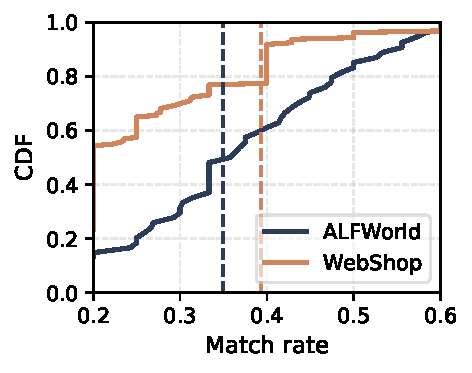
\includegraphics[width=\textwidth, valign=t]{figures/motiexps/match_rate_cdf.pdf}
        \vspace{-0.55em}
        \caption{Step-level match.}
        \label{subfig:edge_match_cdf}
    \end{subfigure}
    % \hfill
    \begin{subfigure}[t]{0.234\textwidth}
        \centering
        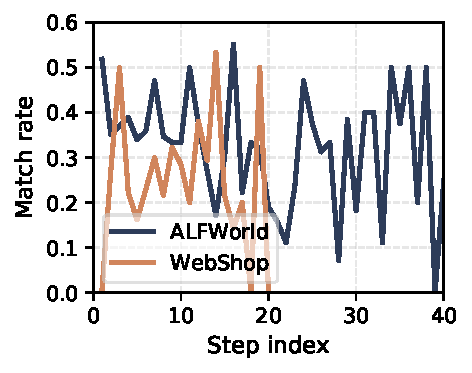
\includegraphics[width=\textwidth, valign=t]{figures/motiexps/step_index.pdf}
        \vspace{-0.55em}
        \caption{Step position.}
        \label{subfig:step_pos}
    \end{subfigure}
    % \hfill
    \begin{subfigure}[t]{0.234\textwidth}
        \centering
        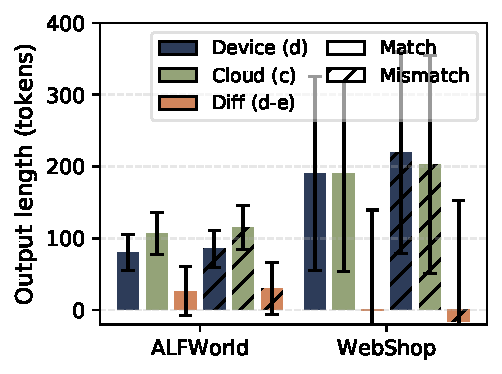
\includegraphics[width=\textwidth, valign=t]{figures/motiexps/thinklength_bar.pdf}
        \caption{Reasoning length.}
        \label{subfig:moti_thinking_length}
    \end{subfigure}
    % \hfill
    \begin{subfigure}[t]{0.234\textwidth}
        \centering
        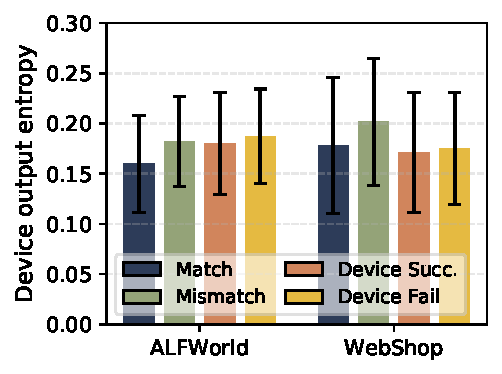
\includegraphics[width=\textwidth, valign=t]{figures/motiexps/entropy_bar.pdf}
        \caption{Predictive entropy.}
        \label{subfig:moti_ent}
    \end{subfigure}\\
    % \vspace{0.5em}
    \begin{subfigure}[t]{0.99\textwidth}
        \centering
        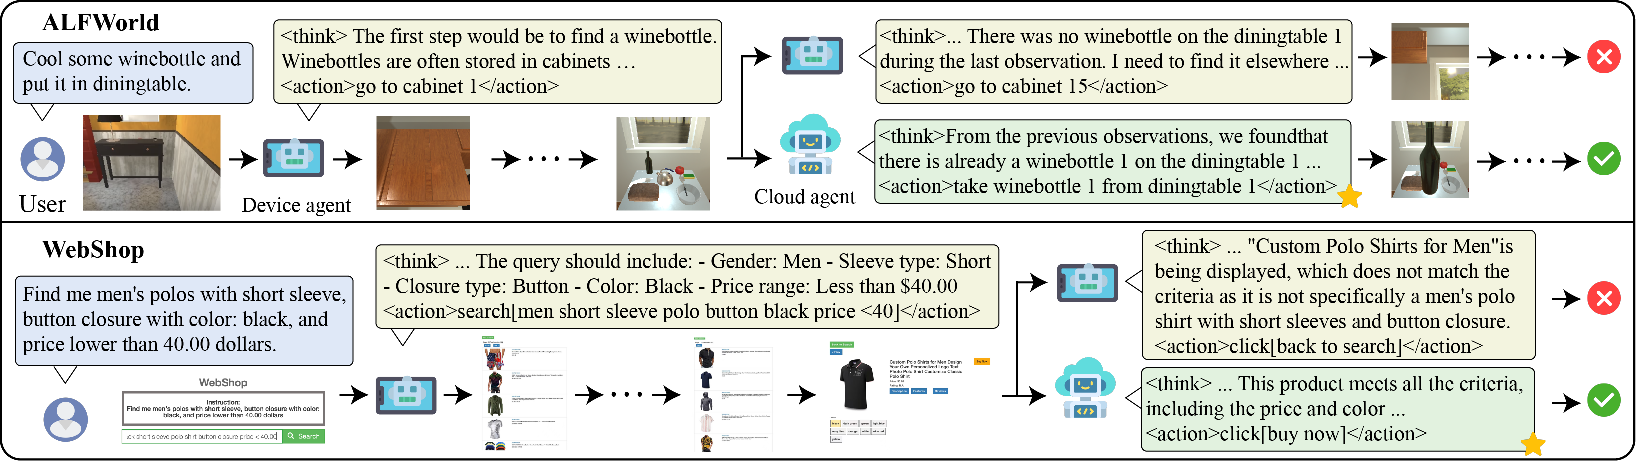
\includegraphics[width=\textwidth, valign=t]{figures/motivating_example.pdf}
        \caption{Example trajectories of device--cloud agents collaboratively solving long-horizon tasks.}
        \label{fig:moti_traj_example}
    \end{subfigure}
    \vspace{-.5em}
    \caption{Step-level performance comparison of device Qwen2.5-7B-Instruct and cloud Qwen-Max on ALFWorld and WebShop tasks.}
    \label{fig:moti_exp_stepwise}
    \vspace{-1.5em}
\end{figure}


% We adopt the ReAct~\citep{Yao2023ReAct} paradigm, where at each step $t$ the agent receives the observation $\mathbf{s}_t$ and outputs both reasoning and action as $\mathbf{a}_t$.
% The reasoning length reflects the depth of deliberation required at each step, while the sequence-level predictive entropy measures model uncertainty, defined as the average token-level entropy:
Figures~\ref{subfig:moti_thinking_length} and~\ref{subfig:moti_ent} quantify the relationship between device--cloud step-level agreement and action difficulty from the perspectives of reasoning length and predictive entropy, respectively.
Reasoning length reflects the depth of deliberation required at each step, while sequence-level predictive entropy captures model uncertainty and is computed as the average token-level entropy:
\begin{equation}
H(\mathbf{a}_t) = -\frac{1}{n} \sum_{i=1}^{n} \sum_{v \in \mathcal{V}} p_\theta(v \mid y_{<i}, \mathbf{s}_t, x) \log p_\theta(v \mid y_{<i}, \mathbf{s}_t, x),
\end{equation}
where $\mathbf{a}_t = (y_1, \dots, y_n) \in \mathcal{V}^n$ is the generated action sequence at step $t$, and $y_{<i} = (y_1, \dots, y_{i-1})$ denotes the token prefix.
The results show that steps with consistent device--cloud outputs are, on average, 13.8 tokens shorter than mismatched ones, indicating a lower required reasoning depth (i.e., more direct and simpler).
Interestingly, the device--cloud reasoning-length gap differs markedly across the two benchmarks.
On ALFWorld, the structured environment and limited action space allow the device model to act more directly, though often without capturing deeper dependencies handled by the cloud. In contrast, WebShop presents a large, unstructured action space—e.g., free-form queries and diverse attribute parsing—causing the weaker device model to produce more verbose deliberation, while the stronger cloud model remains more concise and efficient.
% We find that selectively escalating only a small subset of critical steps to the cloud suffices to recover most of the trajectory-level success. Specifically, routing only the first few reasoning-intensive actions to the cloud while letting the edge model handle the remaining steps achieves over 85\% of the cloud-only trajectory success, with less than 20\% of steps being offloaded.
% In addition to reasoning length, entropy statistics reveal a clear separation: the edge model exhibits higher uncertainty on mismatched steps, while maintaining lower entropy on those aligned with the cloud outputs. This contrast indicates that the need for cloud invocation is not random, but governed by an underlying structure that reflects the intrinsic difficulty of each decision step.
Beyond reasoning length, entropy also exhibits a clear separation: the device model is more uncertain on mismatched steps and more confident on those aligned with the cloud, suggesting that the need for cloud intervention is structured by step difficulty rather than random chance.
% Beyond reasoning length, entropy shows a similar pattern: the device model exhibits higher uncertainty on mismatched steps and lower uncertainty on those aligned with cloud outputs, indicating that the need for cloud intervention is structured rather than random and reflects the intrinsic difficulty of each step.
Moreover, entropy exhibits a similar benchmark-dependent pattern: cloud interventions reduce device entropy on ALFWorld, indicating stronger alignment with device reasoning, but increase it on WebShop, where cloud decisions more often fall outside the device model’s familiar decision regime.
% We further observe a consistent pattern across both benchmarks: multi-turn tasks tend to become simpler as they progress. Early steps often involve complex reasoning, planning, or environment exploration, where the edge model frequently fails. Later steps, by contrast, are often deterministic or involve straightforward execution conditioned on the early decisions, allowing the edge model to succeed without cloud assistance. This temporal structure suggests a natural opportunity for step-wise routing policies: prioritize cloud resources for the front-loaded, high-complexity decisions, and rely on the edge model for subsequent, lower-complexity steps.

Figure~\ref{fig:moti_traj_example} shows examples of device--cloud step-level agreement, with more cases and analysis provided in Appendix~\ref{appendix:case}.
While the device agent can handle many routine follow-up actions, its gap from the cloud agent is concentrated in decisions requiring deeper context tracking, precise grounding, or complex constraint composition. Accurately identifying these steps could substantially reduce cloud calls while preserving task success, highlighting the promise of step-level coordination.

\section{\name: A Long-Horizon Device--Cloud LLM Agent Coordinator}
\label{sec:hera}

This section presents \name, a step-level device--cloud agent coordinator that optimizes Eq.~\ref{eq:opt_obj} to maximize task performance while minimizing cloud reliance.
\name consists of a 500M-parameter decoder-only Transformer with a binary classification head to route between device agent $\pi_{\theta_\mathrm{d}}$ and cloud agent $\pi_{\theta_\mathrm{c}}$. The training of \name follows a two-stage pipeline (pseudocode in Appendix~\ref{append:code}): \textit{a cold-start phase with imitation learning}, followed by \textit{a refinement phase with reinforcement learning}, ultimately enabling effective performance--cost co-optimization in device--cloud LLM agent systems.

\subsection{Cold Start with Imitation Learning}
\label{sec:hera_il}
To equip \name (the coordinator $r_\phi$ in \S~\ref{sec:preliminary}) with initial routing capability, we first employ a cold-start imitation learning (IL) phase. The objective in this stage is to transform the discrete routing decision into a supervised classification problem by identifying the capability gap between device and cloud models across long-horizon trajectories.
For each task $x$, we begin by rolling out both device-side $\pi_{\theta_\mathrm{d}}$ and cloud-side $\pi_{\theta_\mathrm{c}}$ to collect trajectories $\tau_{\mathrm{d}} (x)$ and $\tau_{\mathrm{c}}(x)$, respectively.
Tasks exhibiting the pronounced device--cloud performance gaps are then selected as:
\begin{equation}
X_{\text{diff}} = \left\{ x \;\middle|\; R(\tau_{\mathrm{c}}(x)) - R(\tau_{\mathrm{d}}(x)) > \delta \right\},
\end{equation}
where $\delta$ serves as a prescribed margin of sub-optimality. This set delineates a regime where cloud assistance is fundamentally necessary.
% The remaining tasks are denoted as $X_{\text{undiff}}$, where the device policy achieves near-cloud performance.

Using $X_{\text{diff}}$, we construct step-level supervision signals for $r_\phi$ by using cloud trajectories as an oracle reference, which provide guidance on states where $\pi_{\theta_\mathrm{d}}$ and $\pi_{\theta_\mathrm{c}}$ exhibit discrepancies. 
Specifically, for each $x \in X_{\text{diff}}$, we take cloud rollout 
$\tau_{\mathrm{c}}(x) = \{({\mathbf{s}}^{\mathrm{c}}_t, {\mathbf{a}}_t^{\mathrm{c}})\}_{t=1}^T$, and feed each $({\mathbf{s}}^\mathrm{c}_t,x)$ into $\pi_{\theta_\mathrm{d}}$ to get the corresponding action
% \begin{equation}
$
{\mathbf{a}}_t^{\mathrm{e}} \sim \pi_{\theta_\mathrm{d}}(\cdot \mid {\mathbf{s}}^\mathrm{c}_t,x)
$.
% \end{equation}
We define a step-level consistency indicator as $
% \begin{equation}
y_t = 1- \mathbb{I}\big[{\mathbf{a}}_t^{\mathrm{e}} = {\mathbf{a}}_t^{\mathrm{c}}\big]
% \end{equation}
$, where $y_t=1$ indicates that $\pi_{\theta_\mathrm{d}}$ output disagrees with the cloud oracle and current state should be routed to $\pi_{\theta_\mathrm{c}}$, while $y_t=0$ means $\pi_{\theta_\mathrm{d}}$ is sufficient for local execution.

Based on this, we construct a cold-start IL dataset for the $r_\phi$:
\begin{equation}
\mathcal{D}_{\mathrm{IL}} = \left\{ ({\mathbf{s}}_t, x, y_t) \;\middle|\; x \in X_{\text{diff}},\ ({\mathbf{s}}_t, {\mathbf{a}}_t^{\mathrm{c}}) \in \tau_{\mathrm{c}}(x) \right\}.
\end{equation}
The coordinator $r_\phi$ is then trained as a binary classifier on $\mathcal{D}_{\mathrm{IL}}$ with input $({\mathbf{s}}_t, x)$ and label $y_t$ (as defined in \S~\ref{sec:preliminary}) using a binary cross-entropy (BCE) loss:
\begin{equation}
\mathcal{L}_{\text{IL}}(\phi) = - \frac{1}{|\mathcal{D}_{\text{IL}}|} 
\sum_{(\mathbf{s}_t, x, y_t) \in \mathcal{D}_{\text{IL}}} 
\left[ 
y_t \log p_\phi(\mathbf{s}_t, x) 
+ (1 - y_t)\log \big(1 - p_\phi(\mathbf{s}_t, x)\big) 
\right],
\label{eq:il}
\end{equation}
where $p_\phi(\mathbf{s}, x) \in (0,1)$ denotes the Bernoulli parameter of routing policy $r_\phi(\mathbf{s}, x)$.
% , and $\alpha > 1$ is a hyperparameter used to penalize "false negatives" (failing to route when necessary), which are more detrimental to task success than "false positives" (unnecessary cloud calls).
This cold-start IL phase aligns the coordinator’s latent space with the agents' performance differential, providing a stable policy initialization that significantly accelerates the subsequent RL phase.

\begin{figure*}[t]
    \centering
    \vspace{-1.0em}  % 适当调整与标题间距
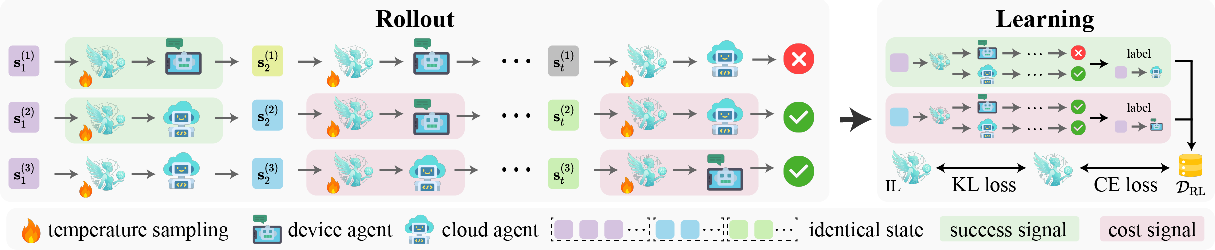
\includegraphics[width=\textwidth,height=8.5cm,keepaspectratio]{figures/rl_training.pdf}
\vspace{-1em}
\caption{RL workflow of \name. We group identical states in multiple rollouts, and derive cost-aware preference labels that favor higher return and fewer future cloud calls to update \name.}
\label{fig:hera_training_overview}
    \vspace{-1.5em}  % 控制与正文间距
\end{figure*}

\subsection{Cost-Aware Reinforcement Learning with State Grouping}
\label{sec:hera_rl}
The IL phase provides a strong initialization but relies on a proxy objective and does not directly optimize Eq.~\ref{eq:opt_obj}. We then refine \name with reinforcement learning (RL)\footnote{We use trajectory return and cost as reinforcement signals, but optimize the router through induced step-level classification targets rather than direct policy gradients.}, jointly maximizing end-to-end task success while minimizing step-level cloud invocations.
We deploy device agent $\pi_{\theta_\mathrm{d}}$ and cloud agent $\pi_{\theta_\mathrm{c}}$, together with router $r_\phi$ trained in the preceding IL stage, into the environment and collect $N$ trajectories for each task $x$ from the same initial state.
To induce sufficient exploration, we sample routing decisions from a temperature-scaled Bernoulli distribution parameterized by the router's binary head.
Concretely, at step $t$ the router $r_\phi$ outputs a logit $\ell_\phi(\mathbf{s}_t,x)$, and we form:
\begin{equation}
p_t^{(\gamma)} \;=\; \sigma\!\left(\ell_\phi(\mathbf{s}_t,x)/\gamma\right),
\qquad
r_{\phi}(\mathbf{s}_t,x) \sim \mathrm{Bernoulli}\!\left(p_t^{(\gamma)}\right),
\label{eq:temperature}
\end{equation}
where temperature $\gamma>0$ (larger $\gamma$ increases stochasticity).
This yields $N$ trajectories $\{\tau_i\}_{i=1}^N$, where each is defined as
\(\tau_i = \{(\mathbf{s}_1^{(i)}, \hat{\mathbf{a}}_1^{(i)} ,r_1^{(i)}), (\mathbf{s}_2^{(i)}, \hat{\mathbf{a}}_2^{(i)} ,r_2^{(i)}), \dots, (\mathbf{s}_T^{(i)}, \hat{\mathbf{a}}_T^{(i)} ,r_T^{(i)})\}\). All trajectories share the same initial state, i.e., $\mathbf{s}_1^{(1)}=\mathbf{s}_1^{(2)}=,\cdots,=\mathbf{s}_1^{(N)}$.

We then group identical states to derive step-level learning signals.
Let $\mathcal{G}(x)$ denote the set of distinct states encountered across the $N$ trajectories.
For each grouped state $\mathbf{s}\in\mathcal{G}(x)$, we collect all its occurrences
$
\mathcal{J}(\mathbf{s}) \coloneqq \{\, (i,t) \mid \mathbf{s}^{(i)}_t=\mathbf{s} \,\},
$
which enumerates every visit to $\mathbf{s}$.
For each $\mathbf{s}\in\mathcal{G}(x)$, we estimate two quantities conditioned on the routing decision:
(1) the expected trajectory return, and
(2) the expected future cloud reliance.
Specifically, we compute decision-conditioned averages by restricting $r_{\phi} ({\mathbf{s}}_{t}^{(i)},x)=d$:
\begin{align}
\widehat{R}(d;\mathbf{s})
&:= \frac{1}{\sum_{(i,t)\in\mathcal{J}(\mathbf{s})}\mathbb{I}[r_{\phi} ({\mathbf{s}}_{t}^{(i)},x)=d]}
\sum_{(i,t)\in\mathcal{J}(\mathbf{s})}\mathbb{I}[r_{\phi} ({\mathbf{s}}_{t}^{(i)},x)=d]\; R(\tau_i), \label{eq:group_return2}\\
\widehat{C}(d;\mathbf{s})
&:= \frac{1}{\sum_{(i,t)\in\mathcal{J}(\mathbf{s})}\mathbb{I}[r_{\phi} ({\mathbf{s}}_{t}^{(i)},x)=d]}
\sum_{(i,t)\in\mathcal{J}(\mathbf{s})}\mathbb{I}[r_{\phi} ({\mathbf{s}}_{t}^{(i)},x)=d]\; C_{i,t}, \label{eq:group_cloud2}
\end{align}
for $d\in\{0,1\}$, where $d=0$ routes to $\pi_{\theta_\mathrm{d}}$ and $d=1$ routes to $\pi_{\theta_\mathrm{c}}$.
Here, $\widehat{R}(d;\mathbf{s})$ estimates the expected trajectory return, and $\widehat{C}(d;\mathbf{s})$ estimates the expected remaining cloud calls (including the current step), where
$C_{i,t} := \sum_{t' = t}^{T} \mathbb{I}\!\left[r_{\phi} ({\mathbf{s}}_{t'}^{(i)},x) = 1\right]$.

We use above estimates to derive a cost-aware routing rule for step-level supervision.
For each $\mathbf{s}\in\mathcal{G}(x)$, we define a preference label $y(\mathbf{s})\in\{0,1\}$ by selecting the decision with higher estimated return, and breaking near-ties by lower expected cloud usage.
Formally, with a margin $\epsilon>0$:
\begin{equation}
y(\mathbf{s}) :=
\begin{cases}
1, & \widehat{R}(1;\mathbf{s}) - \widehat{R}(0;\mathbf{s}) > \epsilon,\\
0, & \widehat{R}(0;\mathbf{s}) - \widehat{R}(1;\mathbf{s}) > \epsilon,\\
\arg\min\limits_{d\in\{0,1\}} \widehat{C}(d;\mathbf{s}), & \text{otherwise}.
\end{cases}
\label{eq:rl_label_rule}
\end{equation}
Here, $\epsilon$ controls the performance--cost trade-off: $\epsilon\!\to\!0$ favors higher $\widehat{R}$, while $\epsilon\!\to\!+\infty$ favors lower $\widehat{C}$.
In each RL iteration, we roll out $N$ trajectories and construct training set $\mathcal{D}_{\mathrm{RL}}=\{(\mathbf{s},x,y(\mathbf{s})) \mid \mathbf{s}\in\mathcal{G}(x)\}$, and update $r_{\phi}$  by minimizing the BCE loss over $\mathcal{D}_{\mathrm{RL}}$:
\begin{equation}
\mathcal{L}_{\mathrm{RL}}(\phi)
=
-
\frac{1}{|\mathcal{D}_{\mathrm{RL}}|}
\sum_{(\mathbf{s},x,y)\in\mathcal{D}_{\mathrm{RL}}}
\left[
y \log p_{\phi}(\mathbf{s},x)
+
(1-y)\log\big(1-p_{\phi}(\mathbf{s},x)\big)
\right]
+
\beta \, \|\phi-\phi_{\mathrm{IL}}\|_2^2,
\label{eq:rl_loss}
\end{equation}
where $\phi_{\mathrm{IL}}$ is the frozen router parameters obtained at the end of the imitation learning stage, and $\beta$ controls the regularization strength. This regularization stabilizes RL refinement by preventing \name from drifting excessively far from the well-initialized IL stage.

In general, the IL stage provides \name with a strong device--cloud coordination prior, and RL refines it into a cost-aware routing policy that directly optimizes task success under limited cloud usage. Together, \name achieves effective success--cost co-optimization in device--cloud LLM agent systems.

\begin{table}[t]
\centering
\caption{Task success rate, cloud LLM API cost, and end-to-end trajectory latency on ALFWorld, WebShop, and AppWorld, averaged over three runs.}
\label{tab:results}
\vspace{1mm}
\scriptsize
\setlength{\tabcolsep}{2.6pt}
\renewcommand{\arraystretch}{0.95}
\begin{tabular}{l ccc | ccc | ccc}
\toprule
\multirow{2}{*}{\textbf{Method}} 
& \multicolumn{3}{c|}{\textbf{ALFWorld}} 
& \multicolumn{3}{c|}{\textbf{WebShop}} 
& \multicolumn{3}{c}{\textbf{AppWorld}} \\
& Succ. (\%) & Cost ($10^{\scriptstyle -3}\,\$$) & Time (s) 
& Succ. & Cost & Time 
& Succ. & Cost & Time \\
\midrule
Device-only & $48.6_{\pm 1.9}$ & $0.0_{\pm 0.0}$ & $123.0_{\pm 9.1}$ 
          & $3.8_{\pm 0.2}$ & $0.0_{\pm 0.0}$ & $61.8_{\pm 2.5}$ 
          & $0.6_{\pm 0.2}$ & $0.0_{\pm 0.0}$ & $144.2_{\pm 7.4}$ \\
Cloud-only & $90.9_{\pm 0.8}$ & $11.7_{\pm 0.5}$ & $174.1_{\pm 4.9}$ 
           & $35.6_{\pm 1.0}$ & $14.7_{\pm 0.5}$ & $181.5_{\pm 6.3}$ 
           & $22.6_{\pm 1.6}$ & $43.8_{\pm 1.2}$ & $332.5_{\pm 10.3}$ \\
Rand. ($0.3$) & $72.1_{\pm 5.0}$ & $6.1_{\pm 0.2}$ & $157.6_{\pm 7.7}$ 
                              & $21.2_{\pm 1.3}$ & $5.8_{\pm 0.4}$ & $85.9_{\pm 3.4}$ 
                              & $2.4_{\pm 0.4}$ & $14.7_{\pm 0.3}$ & $304.1_{\pm 8.1}$ \\
Rand. ($0.4$) & $77.9_{\pm 4.7}$ & $7.2_{\pm 0.6}$ & $148.1_{\pm 10.5}$ 
                              & $24.5_{\pm 0.8}$ & $6.9_{\pm 0.6}$ & $97.6_{\pm 7.3}$ 
                              & $7.1_{\pm 0.5}$ & $19.2_{\pm 1.4}$ & $363.4_{\pm 13.2}$ \\
Rand. ($0.5$) & $79.1_{\pm 1.5}$ & $8.9_{\pm 1.1}$ & $169.5_{\pm 13.2}$ 
                              & $27.6_{\pm 1.1}$ & $8.3_{\pm 0.7}$ & $108.1_{\pm 4.2}$ 
                              & $5.4_{\pm 0.7}$ & $22.5_{\pm 1.1}$ & $392.7_{\pm 15.7}$ \\
Eagle    & $80.3_{\pm 3.6}$ & $8.5_{\pm 0.4}$ & $178.5_{\pm 6.3}$ 
         & $26.6_{\pm 3.0}$ & $8.0_{\pm 0.9}$ & $116.6_{\pm 2.9}$ 
         & $9.8_{\pm 1.4}$ & $18.2_{\pm 2.5}$ & $317.1_{\pm 14.4}$ \\
Hybrid~LLM  & $79.3_{\pm 1.1}$ & $7.9_{\pm 1.3}$ & $130.2_{\pm 5.8}$     & $29.1_{\pm 3.1}$ & $7.7_{\pm 0.8}$ & $109.3_{\pm 5.1}$ 
         & $16.2_{\pm 0.7}$ & $36.9_{\pm 2.3}$ & $301.9_{\pm 12.5}$ \\
RouteLLM & $83.6_{\pm 2.8}$ & $9.0_{\pm 0.8}$ & $156.7_{\pm 3.3}$
         & $31.1_{\pm 2.6}$ & $7.2_{\pm 0.3}$ & $155.1_{\pm 13.9}$ 
         & $17.6_{\pm 1.9}$ & $31.3_{\pm 4.2}$ & $266.3_{\pm 7.2}$ \\
FrugalGPT & $83.7_{\pm 1.4}$ & $8.7_{\pm 2.1}$ & $203.7_{\pm 4.7}$ 
         & $31.8_{\pm 1.3}$ & $12.1_{\pm 1.1}$ & $125.8_{\pm 8.8}$
         & $18.5_{\pm 2.7}$ & $37.5_{\pm 1.9}$ & $359.5_{\pm 19.3}$ \\
\cellcolor{blue!10}\name& \cellcolor{blue!10}$86.1_{\pm 3.2}$ & \cellcolor{blue!10}$4.0_{\pm 0.9}$ & \cellcolor{blue!10}$105.5_{\pm 5.3}$ 
         & \cellcolor{blue!10}$34.1_{\pm 2.2}$  & \cellcolor{blue!10}$8.1_{\pm 0.6}$ & \cellcolor{blue!10}$112.2_{\pm 4.4}$ 
         & \cellcolor{blue!10}$19.7_{\pm 1.3}$ & \cellcolor{blue!10}$31.3_{\pm 2.6}$ & \cellcolor{blue!10}$286.0_{\pm 9.8}$ \\
\bottomrule
\end{tabular}
\label{table:overall_text}
\vspace{-1em}  % 控制与正文间距
\end{table}

% \begin{table}[t]
% \centering
% \caption{Task success rate and cloud LLM cost on ALFWorld, WebShop, and \needrev{xx}, averaged over three random seeds.
% \needrev{GiGPO$_{\text{w/ std}}$ denotes using $F_{\text{norm}} = \text{std}$, while GiGPO$_{\text{w/o std}}$ uses $F_{\text{norm}} = 1$.}}
% \label{tab:results}
% \vspace{2mm}
% \small
% % \setlength{\tabcolsep}{6.5pt} % 进一步增加列间距使表格布局更美观
% \begin{tabular}{l cc | cc | cc}
% \toprule
% \multirow{2}{*}{\textbf{Method}} & \multicolumn{2}{c|}{\textbf{ALFWorld}} & \multicolumn{2}{c|}{\textbf{WebShop}} & \multicolumn{2}{c}{\textbf{\needrev{xxxx-QA}}} \\
%  & Succ. (\%) & Cost ($10^{\scriptstyle -3}\,\$$) & Succ. & Cost & Succ. & Cost \\
% \midrule
% Edge-only & $48.6_{\pm 1.9}$ & $0.0_{\pm 0.0}$ & $3.8_{\pm x.x}$ & $0.0_{\pm 0.0}$ & $xx.x_{\pm x.x}$ & $0.0_{\pm 0.0}$ \\
% Cloud-only & $90.9_{\pm 0.8}$ & $11.7_{\pm 0.5}$ & $35.6_{\pm x.x}$ & 11.3 & 23.1 & 5.2 \\
% Random ($p_{\mathrm{c}}=0.3$) & $72.1_{\pm 5.0}$ & $6.1_{\pm 0.2}$ & 55.8 & 21.9 & 23.1 & 5.2 \\
% Random ($p_{\mathrm{c}}=0.4$) & $77.9_{\pm 4.7}$ & $7.2_{\pm 0.5}$ & 55.8 & 21.9 & 23.1 & 5.2 \\
% Random ($p_{\mathrm{c}}=0.5$) & $79.1_{\pm 1.5}$ & $8.9_{\pm 0.2}$ & 55.8 & 21.9 & 23.1 & 5.2 \\
% % Random ($p_{\mathrm{c}}=0.75$) & 21.8 & - & 55.8 & 21.9 & 23.1 & 5.2 \\
% Eagle & \needrev{$54.4_{\pm 3.1}$} & - & $73.8_{\pm 3.0}$ & $51.5_{\pm 2.9}$ & 23.1 & 5.2 \\
% RouteLLM & \needrev{$54.4_{\pm 3.1}$} & - & $73.9_{\pm 5.6}$ & $52.1_{\pm 6.7}$ & 23.1 & 5.2 \\
% MinionS & \needrev{$54.4_{\pm 3.1}$} & - & $75.8_{\pm 3.5}$ & $56.8_{\pm 3.8}$ & 23.1 & 5.2 \\
% % \textbf{GiGPO$_{\text{w/ std}}$} & \needrev{$54.4_{\pm 3.1}$} & - & $83.1_{\pm 1.6}$ & $65.0_{\pm 3.2}$ & 23.1 & 5.2 \\
% % \textbf{GiGPO$_{\text{w/o std}}$} & \needrev{$54.4_{\pm 3.1}$} & - & $\mathbf{83.5}_{\pm 1.8}$ & 23.1 & 5.2 & $\mathbf{67.4}_{\pm 4.5}$ \\
% \cellcolor{blue!10}\name & \needrev{$54.4_{\pm 3.1}$} & - & $\mathbf{83.5}_{\pm 1.8}$ & 23.1 & 5.2 & $\mathbf{67.4}_{\pm 4.5}$ \\
% \bottomrule
% \end{tabular}
% \label{table:overall_text}
% \end{table}

% \vspace{-.5em}
\section{Experiment}
\label{sec:exp}

\vspace{-.5em}
We conduct comprehensive evaluations of \name across diverse agentic tasks to show:
(1) the strong device--cloud coordination capability of \name for an optimal performance--cost trade-off;
(2) the contribution of each training stage through ablation studies;
(3) microbenchmarks, including cloud offloading rate, compute overhead, and analyses of routing patterns.
% We conduct comprehensive evaluations of \name across variety of agentic tasks, aiming to demonstrate:
% (1) the strong capability of \name to coordinate device–cloud LLM agents, achieving an optimal performance–cost trade-off;
% (2) the ablation study of \name;

\vspace{-.5em}
\subsection{Experimental Settings}
\label{subsec:exp_set}

\vspace{-.5em}
\paragraph{Benchmarks.}
We evaluate \name on three challenging long-horizon agent benchmarks:
ALFWorld~\citep{ALFWorld20}, WebShop~\citep{yao2022webshop}, and AppWorld~\citep{appworld}.
ALFWorld is an embodied benchmark with 3,827 tasks across six household activity categories, designed to evaluate multi-step decision-making and interactive control for LLM agents.
WebShop is a web-based benchmark for LLM agents on realistic shopping tasks, featuring over 1.1M products and 12k user instructions in a large, diverse action space.
AppWorld is a high-fidelity multi-app environment with 9 daily apps and 457 APIs, offering 750 interactive coding-centric agent tasks with robust programmatic evaluation via state- and execution-based unit tests.
% ALFWorld is an embodied benchmark comprising 3,827 task instances, designed to evaluate the multi-step decision-making and interactive control of LLM agents in six common household activity categories: Pick \& Place, Examine in Light, Clean \& Place, Heat \& Place, Cool \& Place, and Pick Two \& Place.
% WebShop is a web-based interactive benchmark for evaluating LLM agents on realistic online shopping tasks. It features over 1.1M products and 12k user instructions, yielding a large and diverse action space. Agents interact with a simulated HTML shopping site to search, navigate, and purchase an item that satisfies the instruction.

% \begin{table}
%   \caption{ablation}
%   \label{sample-table}
%   \centering
%   \begin{tabular}{lll}
%     \toprule
%     \multicolumn{2}{c}{Part}                   \\
%     \cmidrule(r){1-2}
%     Name     & Description     & Size ($\mu$m) \\
%     \midrule
%     Dendrite & Input terminal  & $\sim$100     \\
%     Axon     & Output terminal & $\sim$10      \\
%     Soma     & Cell body       & up to $10^6$  \\
%     \bottomrule
%   \end{tabular}
% \end{table}

\vspace{-.5em}
\paragraph{Baselines.}
We compare \name with a range of competitive baselines: 
(1) device-only and cloud-only LLM agents;
(2) stochastic step-level routing that randomly selects between device and cloud agents with predefined probabilities;
(3) state-of-the-art device--cloud LLM routing methods, including Eagle~\citep{Eagle2024}, FrugalGPT~\citep{chen2024frugalgpt}, Hybrid~LLM~\citep{ding2024hybrid}, and RouteLLM~\citep{ongroutellm}.
Eagle retrieves similar historical queries and combines global and local ELO scores~\citep{elo1967proposed} to route each request to the best LLM.
FrugalGPT first routes queries to a device-side model and escalates to a stronger cloud LLM only when a learned scorer deems the response unreliable.
Hybrid~LLM trains a lightweight router to predict query difficulty and dynamically assign each request to device or cloud model.
% \needrev{MinionS~\citep{narayan2025cost} lets the cloud LLM decompose and verify, while the on-device LLM executes subtasks over local context and returns filtered evidence.}
RouteLLM trains a win-prediction router on preference data and routes to the cloud model when its win probability exceeds a threshold.

\vspace{-.5em}
\paragraph{Implementation details.}
We use the Qwen2.5-7B-Instruct~\citep{yang2024qwen25} as the on-device model and the closed-source Qwen-Max API~\citep{qwen2.5-max2025} as the strong cloud oracle, respectively (other model pairs in Appendix~\ref{append:model_pair}).
\name is initialized from the Qwen2.5-0.5B backbone~\citep{yang2024qwen25} and replaces the LM head with a binary classification head, resulting in a 494M-parameter model.
Training is conducted on 2$\times$H100 GPUs, freezing the backbone and updating only the last two attention layers and the classification head (30M parameters).
% \name initializes from Qwen2.5-0.5B and freeze the backbone, training only the \needrev{last two attention layers and the classification head} (30M parameters).
We use AdamW~\citep{loshchilov2018decoupled} optimizer,
with learning rates of $4e-5$ (IL) and 1e$-$5 (RL), batch sizes of 64 (IL) and 256 (RL).
We set $N=8$, $\delta=0.5$, $\gamma=1.3$, $\epsilon=0.05$, and $\beta=0.1$.
After training, we use the MNN inference engine~\citep{alibaba2020mnn} to deploy both \name and device-side LLM on an NVIDIA GeForce RTX 4090 GPU, evaluating end-to-end performance and cost in a realistic device--cloud collaboration setting.
More training and evaluation details are provided in Appendix~\ref{append:exp_set}.

% We use Qwen2.5-1.5B/3B/7B-Instruct [3] as our base models. The weighting
% coefficient ω is set to 1 with no further tuning. For ALFWorld and WebShop, all RL training methods
% (including ours and the baselines) use exactly the same hyperparameter configurations. The rollout
% group size N for group-based RL methods is set to 8. For search-augmented QA, we follow the same
% settings in Search-R1 [58]. We use E5 [70] as the retriever. The rollout group size N is set to 5 and the
% max turn is set to 4. Moreover, we incorporate similarity-based GiGPO, where anchor state grouping
% is performed by grouping two states if their similarity (longest matching subsequence) exceeds the
% threshold of 0.9. Full training settings and hyperparameter details are provided in Appendix E.1.

\vspace{-.5em}
\subsection{Overall Results}
\label{subsec:main_results}
% \paragraph{Performance on text-only agent tasks.}
Table~\ref{table:overall_text} reports the average task success rate and cost of \name and other baselines on ALFWorld, WebShop, and AppWorld benchmark, where cost includes closed-source cloud API fees and end-to-end latency.
The device-side agent yields the smallest latency but the lowest success rates.
By contrast, the cloud-only agent boosts success by 42.3\%/31.8\%/22.0\% on ALFWorld/WebShop/AppWorld, respectively, at a per-task cost of 11.7/14.7/43.8 $\times 10^{-3}$ dollars and a latency increase of 51.1/119.7/188.3 seconds.
A random router dispatches each step to the device or cloud with a fixed probability (cloud-routing probability in parentheses), yielding a naive success--cost trade-off; however, without step-difficulty or model-preference awareness, it is inefficient—raising the cloud-routing probability from 0.3 to 0.5 improves success by only 5.5\% on average while significantly increasing cloud calls, per-task cost, and latency.
% Notably, with 50\% cloud-routing , the cost far exceeds half of cloud-only, as reduced cloud-based long-horizon planning lengthens trajectories and introduces redundant steps.
Notably, reduced cloud-based long-horizon planning lengthens trajectories and introduces redundant steps.
The semantic-similarity-based router Eagle yields modest gains over random routing at comparable cloud usage, but still lags behind training-based methods in complex agentic environments.
Training-based baselines achieve similar results; FrugalGPT performs d better by conditioning routing on device outputs, but incurs extra latency by waiting for device generation.
By contrast, \name consistently outperforms all baselines, achieving higher task success rates under substantially lower cost.
It achieves 92.5\% of the cloud-only success rate with only 53.6\% of the cloud cost and 69.3\% of the end-to-end latency on average.
This gain is mainly attributed to the RL stage, whose end-to-end trajectory-level success--cost optimization enables \name to learn not only state-wise routing decisions but also their interdependence across consecutive steps, ultimately yielding more precise and cost-effective device--cloud coordination.


\begin{table}[t]
\centering
\caption{Ablation results for two-stage training of \name.}
% \label{tab:results}
\vspace{1mm}
\scriptsize
% \setlength{\tabcolsep}{3.3pt}
\renewcommand{\arraystretch}{0.95}
\begin{tabular}{l cc | cc | cc}
\toprule
\multirow{2}{*}{\textbf{Method}} 
& \multicolumn{2}{c|}{\textbf{ALFWorld}} 
& \multicolumn{2}{c|}{\textbf{WebShop}} 
& \multicolumn{2}{c}{\textbf{AppWorld}} \\
& Succ. (\%) & $\pi_{\theta_\mathrm{c}}$ calls
& Succ. & $\pi_{\theta_\mathrm{c}}$ calls 
& Succ. & $\pi_{\theta_\mathrm{c}}$ calls \\
\midrule
Rand. ($0.5$) & $79.1$
         & $14.5$  & $27.6$
         & $7.8$ & $5.4$ & $14.6$ \\
\name w/o RL & $79.9$ (\textcolor{green!50!black}{$\uparrow0.8$})  % \textcolor{red!70!black}
         & $10.6$ (\textcolor{green!50!black}{$\downarrow3.9$})  & $31.1$ (\textcolor{green!50!black}{$\uparrow3.5$})  % \textcolor{red!70!black}
         & $8.2$ (\textcolor{red!70!black}{$\uparrow0.4$})  & $9.2$ (\textcolor{green!50!black}{$\uparrow3.8$})  % \textcolor{red!70!black}
         & $15.1$ (\textcolor{red!70!black}{$\uparrow0.5$}) \\
\name w/o IL  & $83.3$ (\textcolor{green!50!black}{$\uparrow4.2$}) 
         & $9.3$ (\textcolor{green!50!black} {$\downarrow5.2$}) & $29.9$ (\textcolor{green!50!black}{$\uparrow2.3$}) 
         & $7.2$ (\textcolor{green!50!black} {$\downarrow0.6$}) & $14.3$ (\textcolor{green!50!black}{$\uparrow8.9$}) & $17.3$ (\textcolor{red!70!black}{$\uparrow2.7$}) \\
\cellcolor{blue!10}\name 
         & \cellcolor{blue!10}$86.1$ (\textcolor{green!50!black}{$\uparrow7.0$})
         & \cellcolor{blue!10}$5.3$ (\textcolor{green!50!black}{$\downarrow9.2$}) & \cellcolor{blue!10}$34.1$ (\textcolor{green!50!black}{$\uparrow6.5$})
         & \cellcolor{blue!10}$5.1$ (\textcolor{green!50!black}{$\downarrow2.7$}) & \cellcolor{blue!10}$19.7$ (\textcolor{green!50!black}{$\uparrow14.3$}) & \cellcolor{blue!10}$15.7$ (\textcolor{red!70!black}{$\uparrow0.9$}) \\
\bottomrule
\end{tabular}
\label{table:abaltion}
\vspace{-2em}
\end{table}

\begin{wrapfigure}{rB}{0.715\textwidth}
\vspace{-1em}
    \centering
    \begin{subfigure}[t]{0.243\textwidth}
        \centering
        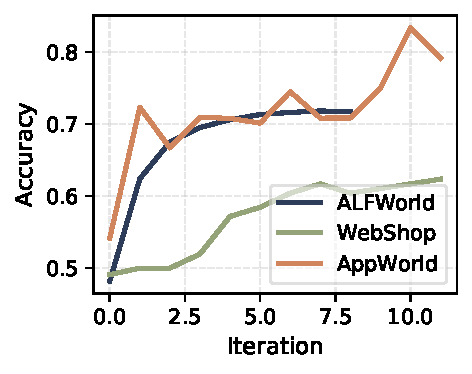
\includegraphics[width=\textwidth, valign=t]{figures/exps/il_progess.pdf}
        \vspace{-.7em}
        \caption{IL stage.}
        \label{subfig:il_progess}
    \end{subfigure}
    % \hfill
    \begin{subfigure}[t]{0.222\textwidth}
        \centering
        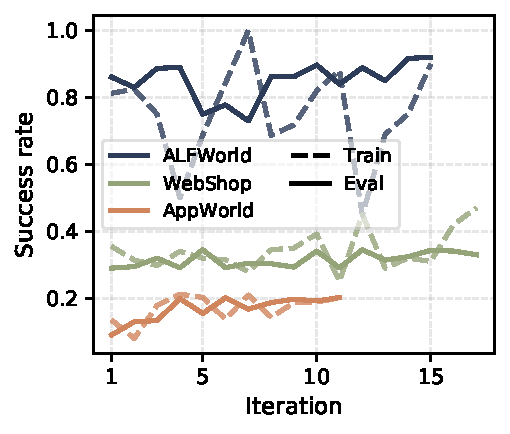
\includegraphics[width=\textwidth, valign=t]{figures/exps/rl_success.pdf}
        \vspace{-0.55em}
        \caption{RL stage (success).}
        \label{subfig:rl_success}
    \end{subfigure}
    \begin{subfigure}[t]{0.222\textwidth}
        \centering
        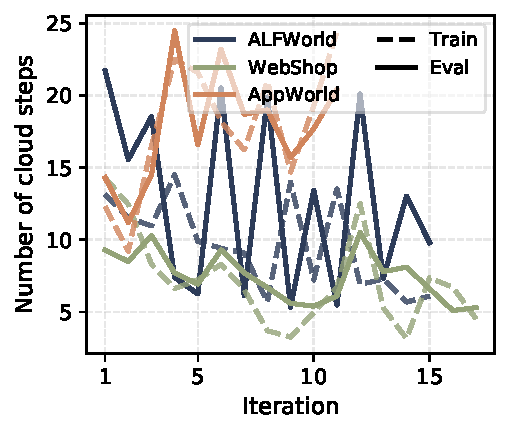
\includegraphics[width=\textwidth, valign=t]{figures/exps/rl_cost.pdf}
        \vspace{-0.55em}
        \caption{RL stage (cost).}
        \label{subfig:rl_cost}
    \end{subfigure}
    \caption{Training dynamics of \name. IL: device--cloud consistency classification accuracy on a held-out validation set. RL: success rate and average cloud invocations on the benchmarks.}
    \label{fig:2_stage_curve}
    \vspace{-1em}
\end{wrapfigure}

\vspace{-.5em}
\subsection{Ablation Study}
\label{subsec:ablation}

Table~\ref{table:abaltion} reports benchmark results after ablating each training stage, including average per-task success rate and cloud-agent call count.
After the IL stage (w/o RL), \name already outperforms the random policy, improving success by 0.8\%/3.5\%/3.8\% on ALFWorld/WebShop/AppWorld while reducing cloud calls by 3.9/-0.4/-0.5 per task. This indicates that replaying cloud trajectories on the device model and using output-consistency supervision yields strong signals for detecting states that require cloud assistance, enabling effective coordination.
With RL refinement, \name further improves success by 6.6\% on average, while reducing cloud calls by 2.6 per task.
This highlights the effectiveness of our cost-aware RL design: in a complex state space, \name learns to identify the critical states where cloud assistance is most needed, achieving higher success with a minimal cloud-invocation budget.
Moreover, RL alone (w/o IL) performs worse than \name, since it lacks a good cold start, confirming that \name benefits from the two-stage IL$\rightarrow$RL training pipeline.

% \begin{figure}
%   \centering
%   \fbox{\rule[-.5cm]{0cm}{4cm} \rule[-.5cm]{4cm}{0cm}}
%   \caption{Sample figure caption.}
% \end{figure}

Figure~\ref{fig:2_stage_curve} further illustrates training dynamics across different stages of \name.
Figure~\ref{subfig:il_progess} shows the cold-start IL learning curve on a held-out validation split of $X_{\text{diff}}$.
Training $r_\phi$ on $\mathcal{D}_{\mathrm{IL}}$ improves routing accuracy to approximately 60\%--80\%, showing that device--cloud action consistency provides a strong and learnable coordination prior.
% During RL refinement, trajectory success increases consistently (Figure~\ref{subfig:rl_reward}) while the number of cloud-invoked steps continues to decrease (Figure~\ref{subfig:rl_cost}).
During RL refinement, \name leverages diverse trajectory rollouts to jointly optimize success and cost: trajectory success steadily improves (Figure~\ref{subfig:rl_success}), while cloud-invoked steps consistently decrease (Figure~\ref{subfig:rl_cost}), except in AppWorld where a slight increase in cloud calls yields substantial success gains.
As a results, \name achieve the highest success rate with the lowest cloud usage, demonstrating the effectiveness of carefully designed learning signals. Additional hyperparameter studies and ablations are provided in Appendix~\ref{appdendix:hyper}.

\vspace{-.5em}
\subsection{Micro-benchmarking}
This section presents micro-benchmarks of \name from multiple perspectives, ncluding the number of cloud-invoked steps, computational overhead, and routing patterns.

\paragraph{Number of cloud steps.}
Figure~\ref{fig:cloud_assist} shows the task success rates of \name and baselines with varying number of cloud-invoked steps.
% Interestingly, under random routing, success increases with an approximately linear trend as more steps are executed by $\pi_{\theta_\mathrm{c}}$.
Under random routing, success grows approximately linearly with the number of steps executed by $\pi_{\theta_\mathrm{c}}$ in ALFWorld and WebShop; interestingly, AppWorld exhibits a noticeable improvement after about 21 cloud calls per trajectory, reflecting its stronger reliance on the cloud model’s coding capability.
Training-based baselines (HybridLLM, RouteLLM, FrugalGPT) outperform random routing but still trail \name, as they rely on static estimates—akin to our IL stage—whereas \name’s cost-aware RL directly optimizes the success--cost trade-off from a holistic trajectory perspective. In comparison, \name achieves superior success rates at equivalent cloud costs and establish a strong Pareto frontier in device--cloud LLM agent systems.
% While training-based baselines (Hybrid~LLM, RouteLLM, FrugalGPT) outperform random routing, they still lag significantly behind \name. This discrepancy stems from their reliance on static estimates—akin to our IL stage—whereas \name’s cost-aware RL directly optimizes the performance–cost trade-off from a holistic trajectory perspective. Consequently, \name achieves superior success rates at equivalent cloud costs, effectively establishing the device–cloud Pareto frontier for long-horizon LLM agents.

\vspace{-.5em}
\paragraph{Computational overhead.}
% Figure~\ref{fig:latency_break} reports a per-task latency breakdown for long-horizon agent tasks when \name coordinates the \needrev{Mac mini} with the cloud-model API.
% Meanwhile, \name attains \needrev{xx\%} of cloud-only success with only \needrev{xx\%} of its latency via efficient device–cloud coordination.
Figure~\ref{fig:latency_break} breaks down per-task latency when \name coordinates the device agent on an NVIDIA RTX 4090 GPU with the cloud-model API, revealing that the end-to-end execution time is predominantly dominated by device and cloud LLM inference.
Notably, deploying \name on device incurs only marginal overhead, adding merely 61ms per step.
As a result, \name attains 95\%/96\%/87\% of cloud-only success on ALFWorld/WebShop/AppWorld, respectively, while incurring only 60\%/62\%/86\% of cloud execution latency via efficient device--cloud coordination.
% Thus, \name proves to be lightweight, with the performance gains from coordination clearly outweighing the negligible on-device overhead.
Thus, \name proves to be exceptionally lightweight; the substantial gains in task success and the overall latency reduction achieved by accurately routing steps to the device outweigh the trivial on-device computational overhead, validating its suitability for real-world, latency-sensitive deployments.

\begin{figure}[t]
\centering
\begin{minipage}[t]{0.73\textwidth}
  \centering
  \begin{subfigure}[t]{0.32\textwidth}
    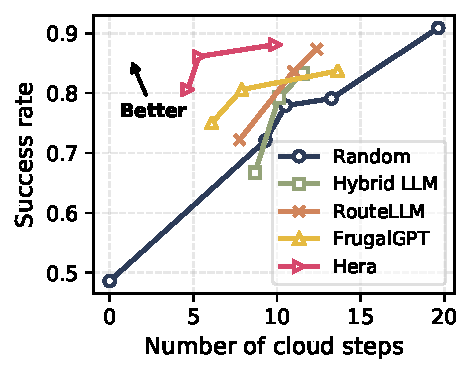
\includegraphics[width=\textwidth]{figures/exps/clouassist_alfworld.pdf}
    \caption{ALFWorld.}
  \end{subfigure}
  \begin{subfigure}[t]{0.32\textwidth}
    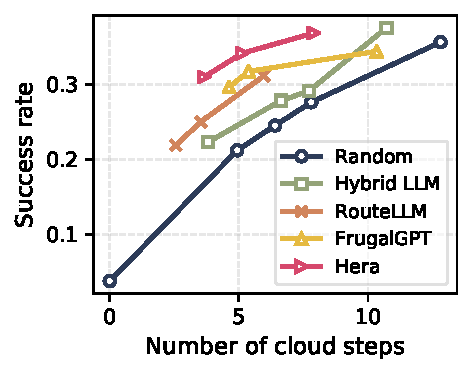
\includegraphics[width=\textwidth]{figures/exps/clouassist_webshop.pdf}
    \caption{WebShop.}
  \end{subfigure}
  \begin{subfigure}[t]{0.32\textwidth}
    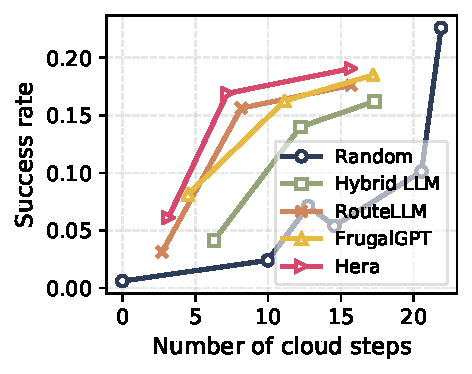
\includegraphics[width=\textwidth]{figures/exps/clouassist_appworld.pdf}
    \caption{AppWorld.}
  \end{subfigure}
  \caption{Task success rate of \name and baselines as a function of cloud invocation count on ALFWorld, WebShop, and AppWorld.}
  \label{fig:cloud_assist}
\end{minipage}\hfill
\begin{minipage}[t]{0.25\textwidth}
  \centering
  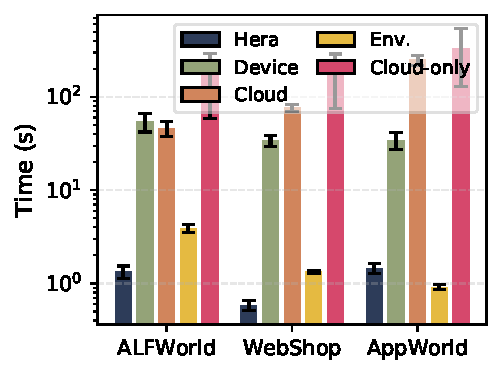
\includegraphics[width=\textwidth]{figures/exps/latency_break.pdf}
  \vspace{-1.7em}
  \caption{End-to-end latency breakdown for device--cloud collaborative LLM agent systems.}
  \label{fig:latency_break}
\end{minipage}
\vspace{-1.5em}
\end{figure}

\begin{wrapfigure}{r}{0.52\textwidth}
\vspace{-1em}
    \centering
    \begin{subfigure}[t]{0.235\textwidth}
        \centering
        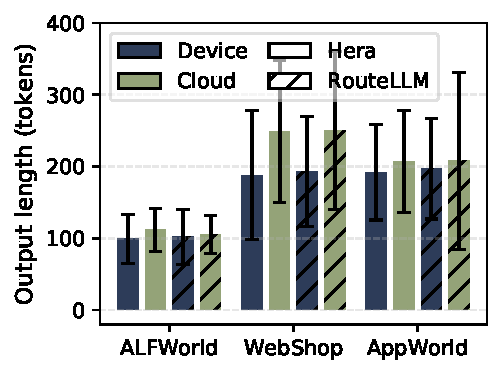
\includegraphics[width=\textwidth, valign=t]{figures/exps/thinklength_bar_exp.pdf}
        \caption{Reasoning length.}
        \label{subfig:333}
    \end{subfigure}
    % \hfill
    \begin{subfigure}[t]{0.235\textwidth}
        \centering
        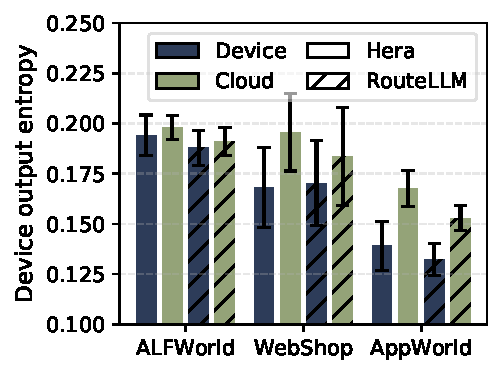
\includegraphics[width=\textwidth, valign=t]{figures/exps/ent_bar_exp.pdf}
        \caption{Predictive entropy.}
        \label{subfig:ent_bar_exp}
    \end{subfigure}
    \caption{Device-side agent output characteristics for device- and cloud-executed steps.}
    \label{fig:moti_exp_stepwise}
\vspace{-1em}
\end{wrapfigure}

\vspace{-.5em}
\paragraph{Routing patterns.}
Following \S~\ref{sec:motivation}, we compare \name with RouteLLM in terms of reasoning length and predictive entropy (replayed on $\pi_{\theta_\mathrm{d}}$) for states with distinct routing decisions in successful trajectories, demonstrating its implicit capture of task difficulty.
Compared to RouteLLM, \name induces a more pronounced separation in both reasoning length and entropy between device- and cloud-executed steps when evaluated on the device agent.
This sharper divergence, together with the success--cost results, indicates that \name more effectively identifies high-uncertainty, cognitively demanding steps, enabling more discriminative and difficulty-aware step-level routing.

% \begin{wrapfigure}{l}{0.7\textwidth}
%     \centering
%     \begin{subfigure}[t]{0.234\textwidth}
%         \centering
%         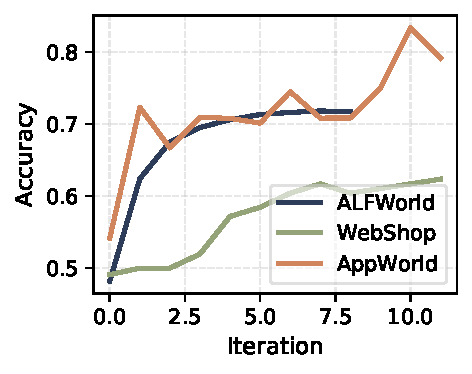
\includegraphics[width=\textwidth, valign=t]{figures/exps/il_progess.pdf}
%         \vspace{-0.55em}
%         \caption{\needrev{ALFWorld}.}
%         \label{subfig:cloud_assist}
%     \end{subfigure}
%     % \hfill
%     \begin{subfigure}[t]{0.234\textwidth}
%         \centering
%         \includegraphics[width=\textwidth, valign=t]{figures/exps/rl_reward.pdf}
%         \vspace{-0.55em}
%         \caption{\needrev{WebShop.}}
%         \label{subfig:latency_break}
%     \end{subfigure}
%     % \hfill
%     \begin{subfigure}[t]{0.234\textwidth}
%         \centering
%         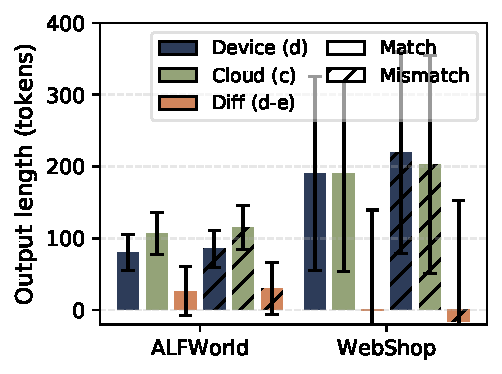
\includegraphics[width=\textwidth, valign=t]{figures/motiexps/thinklength_bar.pdf}
%         \caption{\needrev{AppWorld}.}
%         \label{subfig:333}
%     \end{subfigure}
%     \caption{Task success rate of \name and baselines as a function of cloud invocation count on ALFWorld, WebShop, and AppWorld benchmarks.}
%     \label{fig:moti_exp_stepwise}
% \end{wrapfigure}

% \begin{wrapfigure}{r}{0.25\textwidth}
%     \centering
%     % \vspace{-1.2em}
%     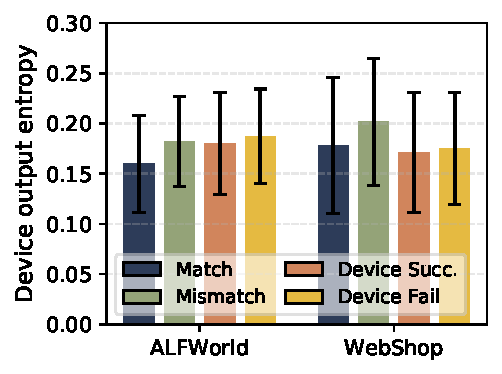
\includegraphics[width=0.25\textwidth]{figures/motiexps/entropy_bar.pdf}
%     \vspace{-0.3em}
%     \caption{\needrev{\name cost-aware rl xxx.}}
%     \label{fig:overhead}
%     % \vspace{-2.0em}
% \end{wrapfigure}


% \begin{figure*}[t]
%     \centering
%     \vspace{-1.0em}  % 适当调整与标题间距
% 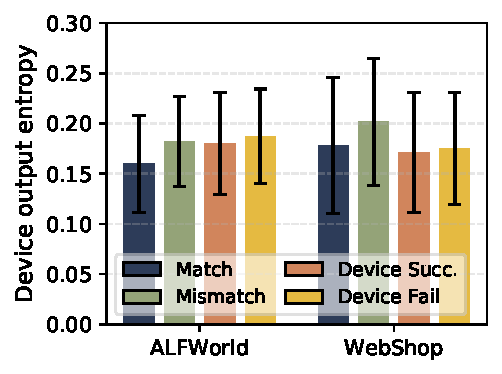
\includegraphics[width=\textwidth,height=2.5cm,keepaspectratio]{figures/motiexps/entropy_bar.pdf}
% \caption{\needrev{\name cost-aware rl xxx.}}
% \label{fig:overhead}
%     % \vspace{-1.0em}  % 控制与正文间距
% \end{figure*}


\section{Conclusions}

This paper proposes \name, a step-level device--cloud LLM agent coordinator for long-horizon tasks. Specifically, \name accurately identifies whether cloud assistance is needed at each interaction state, thus enabling effective task execution with minimal cloud invocations. \name adopts a two-stage training paradigm. First, we perform cold-start imitation learning by replaying the device agent on cloud trajectories and using step-level action consistency as supervision, providing \name with an initial device--cloud routing capability.
Next, we refine \name via cost-aware reinforcement learning: across multiple rollouts, we group identical states and generate step-level preferences that favor higher return and, when comparable, fewer future cloud calls, thereby explicitly co-optimizing success and cost.
Extensive experiments on ALFWorld, WebShop, and AppWorld demonstrate that \name consistently outperforms state-of-the-art baselines while invoking the cloud agent in only 46.3\% of steps and achieving 92.5\% of cloud-only success.
% Extensive experiments on ALFWorld, WebShop, and AppWorld benchmarks validate \name, outperforming state-of-the-art baselines, \needrev{with only 27.1\% cloud-invocation steps and achieving 94.7\% of the cloud-only success rate}.
We present the broader impact of \name in Appendix~\ref{appendix:impact}, and discuss the limitations of \name and directions for future research in Appendix~\ref{appdendix:limit_future}.



\begin{ack}
% \needrev{acknowledgment}
This work was supported by Key Research and Development Program of Zhejiang Province (No. 2025C01026)
\end{ack}

% \section*{References}

{\small
\bibliographystyle{plainnat}
\bibliography{refs}
}

%%%%%%%%%%%%%%%%%%%%%%%%%%%%%%%%%%%%%%%%%%%%%%%%%%%%%%%%%%%%

\newpage
\appendix

% \section{Technical Appendices and Supplementary Material}
% Technical appendices with additional results, figures, graphs and proofs may be submitted with the paper submission before the full submission deadline (see above), or as a separate PDF in the ZIP file below before the supplementary material deadline. There is no page limit for the technical appendices.

\section{Broader Impacts}
\label{appendix:impact}

This work introduces \name as the first step-level device--cloud coordinator for LLM agents, marking a pivotal shift from coarse, task-level routing to fine-grained, dynamic collaboration. By demonstrating that only a small fraction of critical steps require cloud intervention, \name significantly lowers the computational and financial barriers to deploying sophisticated agents on user devices. This efficiency democratizes access to advanced agentic capabilities, enabling real-time, latency-sensitive applications—such as autonomous robotic control and interactive assistants—to operate reliably on device hardware without prohibitive costs.

Amid the explosive growth of LLM agents, artificial intelligence is undergoing a fundamental paradigm shift from static, single-turn queries to long-horizon autonomous interaction, where agents must sustain coherent reasoning over extended, dynamic trajectories. We believe \name is essential for realizing scalable, sustainable, and ubiquitous autonomous agents in real-world applications by establishing a strong performance--cost Pareto frontier for this complex mode of operation.

% \newpage
\section{Pseudocode}
\label{append:code}

Algorithm~\ref{alg:hera} summarizes the 2-stage training procedure of \name.

\begin{algorithm}[h]
\caption{\name:Two-Stage Training for Step-Level Device--Cloud LLM Agent Coordination}
\label{alg:hera}
\begin{algorithmic}[1]
\STATE \textbf{Input:} Device policy $\pi_{\theta_d}$, cloud policy $\pi_{\theta_c}$, router $r_\phi$; margins $\delta,\epsilon$; temperature $\gamma$; rollouts per task $N$; regularization weight $\beta$.
\STATE \textbf{Output:} Trained router parameters $\phi$.

\STATE {\bf Stage I: Cold-start imitation learning}
\STATE Initialize $\mathcal{D}_{\mathrm{IL}} \leftarrow \emptyset$.
\FORALL{tasks $x$}
    \STATE Roll out $\pi_{\theta_d}$ to get $\tau_d(x)$; roll out $\pi_{\theta_c}$ to get $\tau_c(x)$.
    \IF{$R(\tau_c(x)) - R(\tau_d(x)) > \delta$}
        \FOR{$t = 1,2,\ldots,T$}
            \STATE Let $(s_t^c,a_t^c)$ be the $t$-th state--action pair in $\tau_c(x)$.
            \STATE Sample $a_t^d \sim \pi_{\theta_d}(\cdot \mid s_t^c,x)$.
            \STATE $y_t \leftarrow \mathbb{I}[a_t^d = a_t^c]$.
            \STATE $\mathcal{D}_{\mathrm{IL}} \leftarrow \mathcal{D}_{\mathrm{IL}} \cup \{(s_t^c,x,y_t)\}$.
        \ENDFOR
    \ENDIF
\ENDFOR
\STATE Update $\phi$ by minimizing the IL objective $\mathcal{L}_{\mathrm{IL}}(\phi)$ (Eq.~\ref{eq:il}).
\STATE Save $\phi_{\mathrm{IL}} \leftarrow \phi$.

\STATE {\bf Stage II: Cost-aware reinforcement learning with state grouping}
\FOR{each RL iteration}
    \STATE Initialize $\mathcal{D}_{\mathrm{RL}} \leftarrow \emptyset$.
    \FORALL{tasks $x$}
        \STATE Collect $N$ trajectories $\{\tau_i\}_{i=1}^N$ using temperature $\gamma$ (Eq.~\ref{eq:temperature}).
        \STATE Group identical states across $\{\tau_i\}$ to obtain $\mathcal{G}(x)$ and $J(s)$.
        \FORALL{$s \in \mathcal{G}(x)$}
            \STATE Estimate $\widehat{R}(d;s)$ and $\widehat{C}(d;s)$ for $d\in\{0,1\}$ (Eqs.~\ref{eq:group_return2} and~\ref{eq:group_cloud2}).
            \STATE Derive preference label $y(s)$ (Eq.~\ref{eq:rl_label_rule}).
            \STATE $\mathcal{D}_{\mathrm{RL}} \leftarrow \mathcal{D}_{\mathrm{RL}} \cup \{(s,x,y(s))\}$.
        \ENDFOR
    \ENDFOR
    \STATE Update $\phi$ by minimizing $\mathcal{L}_{\mathrm{RL}}(\phi)$ with regularization to $\phi_{\mathrm{IL}}$ (Eq.~\ref{eq:rl_loss}).
\ENDFOR

\RETURN $\phi$.
\end{algorithmic}
\end{algorithm}


% \newpage
\section{Experimental Details}
\label{appendix:exp}
% Technical appendices with additional results, figures, graphs and proofs may be submitted with the paper submission before the full submission deadline (see above), or as a separate PDF in the ZIP file below before the supplementary material deadline. There is no page limit for the technical appendices.

\subsection{Prompts}
The prompts used by LLM agents in ALFWorld, WebShop, and AppWorld are shown below.

\begin{promptbox}[title=Prompt Template for ALFWorld]
\begin{lstlisting}[style=mytt]
You are an expert agent operating in the ALFRED Embodied Environment. Your task is to: {task_description}
Prior to this step, you have already taken {step_count} step(s). Below are the most recent {history_length} observations and the corresponding actions you took: {action_history}
You are now at step {current_step} and your current observation is: {current_observation}
Your admissible actions of the current situation are: [{admissible_actions}].

Now it's your turn to take an action.
You should first reason step-by-step about the current situation. This reasoning process MUST be enclosed within <think> </think> tags. 
Once you've finished your reasoning, you should choose an admissible action for current step and present it within <action> </action> tags.
\end{lstlisting}
\end{promptbox}

\begin{promptbox}[title=Prompt Template for WebShop]
\begin{lstlisting}[style=mytt]
You are an expert autonomous agent operating in the WebShop e-commerce environment.
Your task is to: {task_description}.
Prior to this step, you have already taken {step_count} step(s). Below are the most recent
{history_length} observations and the corresponding actions you took: {action_history}
You are now at step {current_step} and your current observation is: {current_observation}.
Your admissible actions of the current situation are:
[
{available_actions}
].

Now it's your turn to take one action for the current step.
You should first reason step-by-step about the current situation, then think carefully which
admissible action best advances the shopping goal. This reasoning process MUST be enclosed
within <think> </think> tags.
Once you've finished your reasoning, you should choose an admissible action for current step
and present it within <action> </action> tags.
\end{lstlisting}
\end{promptbox}
% \newpage

\begin{promptbox}[title=Prompt Template for AppWorld]
\begin{lstlisting}[style=mytt]
I am your supervisor and you are a super intelligent AI Assistant whose job is to achieve my day-to-day tasks completely autonomously.

To do this, you will need to interact with app/s (e.g., spotify, venmo, etc) using their associated APIs on my behalf. For this you will undertake a *multi-step conversation* using a python REPL environment. That is, you will write the python code and the environment will execute it and show you the result, based on which, you will write python code for the next step and so on, until you've achieved the goal. This environment will let you interact with app/s using their associated APIs on my behalf.

Here are three key APIs that you need to know to get more information

# To get a list of apps that are available to you.
print(apis.api_docs.show_app_descriptions())

# To get the list of apis under any app listed above, e.g. supervisor
print(apis.api_docs.show_api_descriptions(app_name='supervisor'))

# To get the specification of a particular api, e.g. supervisor app's show_account_passwords
print(apis.api_docs.show_api_doc(app_name='supervisor', api_name='show_account_passwords'))

Each code execution will produce an output that you can use in subsequent calls. Using these APIs, you can now generate code, that the environment will execute, to solve the task.

Using these APIs, now begin writing code cells step-by-step to solve the actual task:

My name is: {supervisor_first_name} {supervisor_last_name}. My personal email is {supervisor_email} and phone number is {supervisor_phone_number}.

Your task is: {task_description}

Now it's your turn to generate code to solve the task.
You should first reason step-by-step about which APIs to call, what arguments to use, and how to build your code block to complete the task. This reasoning process MUST be enclosed within <think> </think> tags.
Once you've finished your reasoning, you present the solution code body within <code> </code> tags.
\end{lstlisting}
\end{promptbox}

\subsection{Details of Experimental Settings}
\label{append:exp_set}

% \paragraph{Hyperparameters for ALFWorld.}
For ALFWorld benchamrks ,we use a maximum prompt length of 2048 tokens and a maximum response length of 512 tokens.
Each episode is capped at 50 environment interaction steps, counting both device- and cloud-executed actions.
In WebShop, the prompt length is capped at 4096 tokens and the response length at 1024 tokens. Each episode terminates after 20 interaction steps.
In AppWorld, we set the maximum prompt length to 4096 tokens, the maximum response length to 1024 tokens, and the maximum number of steps to 50.
At each execution step, the agent is given access to a bounded history window. The number of visible historical steps is set to 50, 15, and 5 for the three datasets, respectively.
% \needrev{Technical appendices with additional results, figures, graphs and proofs may be submitted with the paper submission before the full submission deadline (see above), or as a separate PDF in the ZIP file below before the supplementary material deadline. There is no page limit for the technical appendices.}
% \paragraph{Hyperparameters for AppWorld.}
% \paragraph{Implementation of baselines.}
To evaluate request-level baselines in long-horizon agent settings, we apply them independently at each interaction step. Specifically, at step $t$, each baseline receives the same per-step context as \name—task instruction, current observation, and truncated history—and outputs a binary decision for routing the current step to either the device or the cloud model.

The definition of an identical state in the RL training stage depends on the benchmark-specific environment representation. In ALFWorld, two states are considered identical if they correspond to the same textual environment observation and admissible action set. In WebShop, two states are considered identical if they have the same webpage observation, including the current page content and available actions. In AppWorld, two states are considered identical if they produce the same execution observation returned by the Python environment under the same task context.

% \paragraph{Implementation Details.}
For device-side model deployment, we run the open-source MNN engine~\citep{alibaba2020mnn} on a single NVIDIA RTX 4090 GPU using BF16 precision. Cloud-side closed-source models are invoked exclusively through their official APIs. All training experiments are performed on 2 NVIDIA H100 GPUs. Unless otherwise specified, the imitation learning and reinforcement learning phases are run for 30 and 50 iterations, respectively. In practice, however, we observe that the best-performing checkpoint typically emerges much earlier, after only around 10 IL iterations and 15 RL iterations, highlighting the training efficiency of \name.


% \subsection{\needrev{VL-tasks}}
% Technical appendices with additional results, figures, graphs and proofs may be submitted with the paper submission before the full submission deadline (see above), or as a separate PDF in the ZIP file below before the supplementary material deadline. There is no page limit for the technical appendices.

\subsection{Generalization across Device--Cloud Model Pairs}
\label{append:model_pair}
We further validate \name’s generalizability across diverse device--cloud model pairs on ALFWorld benchmark.
Beyond the default pairing of Qwen2.5-7B-Instruct (device) and Qwen-Max (cloud), we additionally use Llama 3.1 8B Instruct~\citep{llama31} as an alternative device model and GPT-5.4~\citep{gpt5-4} as a cloud model, and evaluate all device--cloud combinations formed from these models.
The results in Table~\ref{table:model_pair} demonstrate that \name consistently outperforms baselines across all model pairs, maintaining a superior performance--cost trade-off regardless of the underlying LLM architectures. While absolute success rates and costs vary depending on the capability gap between the specific device and cloud models, \name effectively adapts its routing policy to exploit the complementary strengths of each pair. This confirms that \name’s two-stage training paradigm is model-agnostic and robust, enabling flexible deployment in heterogeneous device--cloud collaborative environments.

\begin{table}[h]
\centering
\caption{Task success rate, cloud LLM API cost, and end-to-end trajectory latency on ALFWorld across different device--cloud model pairs, averaged over three runs.}
% \label{tab:results}
\vspace{1mm}
\scriptsize
\setlength{\tabcolsep}{2.6pt}
\renewcommand{\arraystretch}{0.95}
\begin{tabular}{l ccc | ccc | ccc}
\toprule
\multirow{2}{*}{\textbf{Method}} 
& \multicolumn{3}{c|}{\textbf{Qwen2.5 7B ($\pi_{\theta_\mathrm{d}}$) and GPT‑5.4 ($\pi_{\theta_\mathrm{c}}$)}} 
& \multicolumn{3}{c|}{\textbf{Llama 3.1 8B and Qwen-Max}} 
& \multicolumn{3}{c}{\textbf{Llama 3.1 8B and GPT-5.4}} \\
& Succ. (\%) & Cost ($10^{\scriptstyle -3}\,\$$) & Time (s) 
& Succ. & Cost & Time 
& Succ. & Cost & Time \\
\midrule
Device-only & $48.6_{\pm 1.9}$ & $0.0_{\pm 0.0}$ & $123.0_{\pm 9.1}$ 
          & $28.9_{\pm 1.2}$ & $0.0_{\pm 0.0}$ & $141.0_{\pm 7.3}$ 
          & $28.9_{\pm 1.2}$ & $0.0_{\pm 0.0}$ & $141.0_{\pm 7.3}$ \\
Cloud-only & $93.6_{\pm 0.6}$ & $68.8_{\pm 3.1}$ & $151.1_{\pm 13.2}$ 
           & $90.9_{\pm 0.8}$ & $11.7_{\pm 0.5}$ & $174.1_{\pm 14.9}$  
           & $93.6_{\pm 0.6}$ & $68.8_{\pm 3.1}$ & $151.1_{\pm 13.2}$ \\
Rand. ($0.3$) & $73.2_{\pm 4.4}$ & $35.0_{\pm 5.1}$ & $141.2_{\pm 8.6}$
                              & $47.2_{\pm 1.8}$ & $6.5_{\pm 0.4}$ & $149.0_{\pm 10.4}$ 
                              & $51.3_{\pm 2.9}$ & $31.0_{\pm 2.4}$ & $144.2_{\pm 10.1}$ \\
Rand. ($0.4$) & $78.1_{\pm 4.9}$ & $45.6_{\pm 2.7}$ & $149.7_{\pm 5.9}$
                              & $58.5_{\pm 0.7}$ & $7.1_{\pm 0.7}$ & $155.1_{\pm 7.4}$ 
                              & $63.3_{\pm 5.2}$ & $38.8_{\pm 2.6}$ & $133.3_{\pm 5.9}$ \\
Rand. ($0.5$) & $79.0_{\pm 2.2}$ & $47.8_{\pm 4.6}$ & $153.8_{\pm 8.8}$
                              & $62.3_{\pm 3.1}$ & $9.1_{\pm 0.9}$ & $164.6_{\pm 6.2}$ 
                              & $69.9_{\pm 4.8}$ & $44.3_{\pm 4.5}$ & $142.2_{\pm 15.3}$ \\
Eagle    & $81.2_{\pm 6.5}$ & $50.4_{\pm 6.3}$ & $161.2_{\pm 13.9}$
         & $75.7_{\pm 2.9}$ & $8.4_{\pm 1.1}$ & $175.3_{\pm 6.0}$ 
         & $73.2_{\pm 4.9}$ & $41.7_{\pm 3.8}$ & $162.3_{\pm 9.0}$ \\
Hybrid~LLM   & $76.2_{\pm 4.7}$ & $46.3_{\pm 2.9}$ & $129.2_{\pm 8.5}$ 
         & $76.8_{\pm 4.1}$ & $8.1_{\pm 0.8}$ & $127.7_{\pm 4.4}$ 
         & $76.7_{\pm 3.6}$ & $39.3_{\pm 7.7}$ & $129.4_{\pm 7.1}$ \\
RouteLLM  & $85.5_{\pm 3.1}$ & $52.3_{\pm 4.3}$ & $144.7_{\pm 12.1}$
         & $81.8_{\pm 3.5}$ & $8.9_{\pm 1.0}$ & $145.3_{\pm 7.1}$ 
         & $85.2_{\pm 2.5}$ & $37.2_{\pm 5.2}$ & $172.6_{\pm 16.8}$ \\
FrugalGPT & $88.6_{\pm 4.0}$ & $47.2_{\pm 2.9}$ & $195.5_{\pm 19.2}$
         & $82.4_{\pm 4.0}$ & $8.3_{\pm 0.7}$ & $210.3_{\pm 15.9}$ 
         & $87.3_{\pm 3.7}$ & $36.2_{\pm 1.7}$ & $199.3_{\pm 14.3}$ \\
\cellcolor{blue!10}\name 
         & \cellcolor{blue!10}$89.3_{\pm 2.6}$ & \cellcolor{blue!10}$23.5_{\pm 4.0}$ & \cellcolor{blue!10}$107.8_{\pm 7.8}$ 
         & \cellcolor{blue!10}$83.3_{\pm 5.4}$ & \cellcolor{blue!10}$5.3_{\pm 0.3}$ & \cellcolor{blue!10}$101.2_{\pm 7.6}$ 
         & \cellcolor{blue!10}$88.5_{\pm 4.2}$ & \cellcolor{blue!10}$26.8_{\pm 2.2}$ & \cellcolor{blue!10}$129.6_{\pm 9.5}$ \\
\bottomrule
\end{tabular}
\label{table:model_pair}
\vspace{-1em}  % 控制与正文间距
\end{table}


\subsection{Effect of Hyperparameters}
\label{appdendix:hyper}
We investigate the sensitivity of \name to the  hyperparameter $\epsilon$ and $\beta$. $\epsilon$ governs the trade-off between task success and cloud cost in the RL stage: a small $\epsilon$ (e.g., 0) prioritizes success but incurs excessive cloud usage, while a large $\epsilon$ (e.g., 0.3) overly restricts offloading, leading to performance degradation. Similarly, $\beta$ stabilizes RL updates against the IL initialization; removing regularization ($\beta=0$) causes policy drift, whereas excessive regularization ($\beta$=0.3) hinders adaptation to RL objectives.
Empirical results in Table~\ref{table:hyper} indicate that the optimal configuration ($\epsilon=0.05$, $\beta=0.1$) effectively balances these dynamics, allowing \name to refine the IL prior into a robust, cost-efficient routing policy. This demonstrates that our design successfully leverages moderate regularization to prevent catastrophic forgetting while utilizing a fine-grained preference margin to identify critical states for cloud intervention, ensuring superior co-optimization of accuracy and efficiency.


% \begin{figure}[h]
%     \centering
%     \begin{subfigure}[t]{0.234\textwidth}
%         \centering
%         \includegraphics[width=\textwidth, valign=t]{figures/exps/rl_alfworld_beta.pdf}
%         % \vspace{-0.55em}
%         \caption{\needrev{alfworld-beta}.}
%         \label{subfig:111}
%     \end{subfigure}
%     % \hfill
%     \begin{subfigure}[t]{0.234\textwidth}
%         \centering
%         \includegraphics[width=\textwidth, valign=t]{figures/exps/rl_webshop_beta.pdf}
%         % \vspace{-0.55em}
%         \caption{\needrev{webshop-beta}.}
%         \label{subfig:222}
%     \end{subfigure}
%     % \hfill
%     \begin{subfigure}[t]{0.234\textwidth}
%         \centering
%         \includegraphics[width=\textwidth, valign=t]{figures/exps/rl_reward.pdf}
%         \caption{\needrev{alfworld-epis}.}
%         \label{subfig:333}
%     \end{subfigure}
%     % \hfill
%     \begin{subfigure}[t]{0.234\textwidth}
%         \centering
%         \includegraphics[width=\textwidth, valign=t]{figures/exps/rl_reward.pdf}
%         \caption{\needrev{webshop-epis}.}
%         \label{subfig:444}
%     \end{subfigure}
%     \vspace{-.5em}
%     \caption{\needrev{Step-level performance comparison of edge Qwen2.5-7B-Instruct and cloud Qwen-Max on ALFWorld and WebShop tasks.}}
%     \label{fig:555}
%     \vspace{-1.5em}
% \end{figure}


\begin{table}[h]
\centering
\caption{Hyperparameter sensitivity of \name on ALFWorld.}
% \label{tab:results}
\vspace{1mm}
\scriptsize
% \setlength{\tabcolsep}{3.3pt}
\renewcommand{\arraystretch}{0.95}
\begin{tabular}{l cc | cc | cc}
\toprule
\multirow{2}{*}{\textbf{Method}} 
& \multicolumn{2}{c|}{\textbf{ALFWorld}} 
& \multicolumn{2}{c|}{\textbf{WebShop}} 
& \multicolumn{2}{c}{\textbf{AppWorld}} \\
& Succ. (\%) & $\pi_{\theta_\mathrm{c}}$ calls
& Succ. & $\pi_{\theta_\mathrm{c}}$ calls 
& Succ. & $\pi_{\theta_\mathrm{c}}$ calls \\
\midrule
\name ($\epsilon=0$, $\beta=0.1$) & $92.6$ (\textcolor{green!50!black}{$\uparrow6.5$})
         & $11.7$ (\textcolor{red!70!black}{$\uparrow6.6$})  & $38.1$ (\textcolor{green!50!black}{$\uparrow12.3$})
         & $15.2$ (\textcolor{red!70!black}{$\uparrow9.9$}) & $21.3$ (\textcolor{green!50!black}{$\uparrow1.6$})
         & $19.4$ (\textcolor{red!70!black}{$\uparrow3.7$}) \\
\name ($\epsilon=0.3$, $\beta=0.1$) & $65.7$ (\textcolor{red!70!black}{$\downarrow20.4$})
         & $2.4$ (\textcolor{green!50!black}{$\downarrow2.9$})   & $11.2$ (\textcolor{red!70!black}{$\downarrow22.9$})
         & $1.6$ (\textcolor{green!50!black}{$\downarrow3.5$}) & $15.1$ (\textcolor{red!70!black}{$\downarrow4.6$})
         & $10.5$ (\textcolor{green!50!black}{$\downarrow5.3$}) \\
\name ($\epsilon=0.05$, $\beta=0$) & $84.0$ (\textcolor{red!70!black}{$\downarrow2.1$})  % \textcolor{red!70!black}
         & $7.7$ (\textcolor{red!70!black}{$\uparrow2.4$})  & $31.9$ (\textcolor{red!70!black}{$\downarrow2.2$})  % \textcolor{red!70!black}
         & $4.9$ (\textcolor{green!50!black}{$\downarrow0.2$}) & $13.2$ (\textcolor{red!70!black}{$\downarrow6.5$})  % \textcolor{red!70!black}
         & $12.1$ (\textcolor{red!70!black}{$\downarrow3.6$})   \\
\name ($\epsilon=0.05$, $\beta=0.3$)  &$79.9$ (\textcolor{red!70!black}{$\downarrow6.2$})  % \textcolor{red!70!black}
         & $4.9$ (\textcolor{green!50!black}{$\downarrow0.4$})  & $29.8$ (\textcolor{red!70!black}{$\downarrow4.3$})  % \textcolor{red!70!black}
         & $4.6$ (\textcolor{green!50!black}{$\downarrow0.5$}) & $17.7$ (\textcolor{red!70!black}{$\downarrow2.0$})  % \textcolor{red!70!black}
         & $16.2$ (\textcolor{red!70!black}{$\uparrow0.5$})  \\
\cellcolor{blue!10}\name ($\epsilon=0.05$, $\beta=0.1$)
         & \cellcolor{blue!10}$86.1$ 
         & \cellcolor{blue!10}$5.3$  & \cellcolor{blue!10}$34.1$
         & \cellcolor{blue!10}$5.1$ & \cellcolor{blue!10}$19.7$ & \cellcolor{blue!10}$15.7$ \\
\bottomrule
\end{tabular}
\label{table:hyper}
% \vspace{-2em}
\end{table}

\section{Case Study}
\label{appendix:case}
This section presents case studies to investigate how \name performs step-level device--cloud coordination in agent tasks.
Concretely, we analyze representative successful trajectories on three benchmarks—ALFWorld, WebShop, and AppWorld—each exhibiting distinct structural properties in terms of action space, reasoning patterns, and feedback signals. For each benchmark, we highlight critical decision points, compare device and cloud behaviors, and demonstrate how \name selectively invokes the cloud only when necessary to preserve task success while minimizing cost.

\subsection{ALFWorld}
The example shows how \name coordinates device- and cloud-side agents on ALFWorld. For routine exploration, the device closely matches the cloud, making local execution sufficient. For critical steps requiring state tracking and long-horizon consistency, the cloud becomes decisive: in Step 19, it avoids the device’s redundant exploration and advances the task. This shows that \name learns to invoke the cloud only for success-critical decisions.

\begin{envbox}[title=Step 1: environment]
\begin{lstlisting}[style=mytt]
-= Welcome to TextWorld, ALFRED! =-
You are in the middle of a room. Looking quickly around you, you see a cabinet 20, a cabinet 19, a cabinet 18, a cabinet 17, a cabinet 16, a cabinet 15, a cabinet 14, a cabinet 13, a cabinet 12, a cabinet 11, a cabinet 10, a cabinet 9, a cabinet 8, a cabinet 7, a cabinet 6, a cabinet 5, a cabinet 4, a cabinet 3, a cabinet 2, a cabinet 1, a coffeemachine 1, a countertop 2, a countertop 1, a diningtable 2, a diningtable 1, a drawer 6, a drawer 5, a drawer 4, a drawer 3, a drawer 2, a drawer 1, a fridge 1, a garbagecan 1, a microwave 1, a sinkbasin 1, a stoveburner 4, a stoveburner 3, a stoveburner 2, a stoveburner 1, and a toaster 1.
Your task is to: cool some winebottle and put it in diningtable.
\end{lstlisting}
\end{envbox}

\begin{herabox}[title=Step 1: Hera decision]
\begin{lstlisting}[style=mytt]
0 (device)
\end{lstlisting}
\end{herabox}

\begin{devicebox}[title=Step 1: device agent output]
\begin{lstlisting}[style=mytt]
<think>
To complete the task of cooling some wine bottle and putting it on the dining table, I need to first locate a wine bottle. Given the options, the most likely place to find a wine bottle would be in one of the cabinets, as they are often used for storing food and beverages. I will start by checking the cabinets, beginning with cabinet 1.
</think>
<action>
go to cabinet 1
</action>
\end{lstlisting}
\end{devicebox}

\begin{cloudbox}[title=Step 1: cloud agent output ((if routed)]
\begin{lstlisting}[style=mytt]
<think>
The task is to cool a winebottle and then place it on the diningtable. The first step would be to find a winebottle. Winebottles are often stored in cabinets, so I should check the cabinets. After finding the winebottle, I will need to cool it, which can be done using the fridge. Finally, after cooling, I will take the winebottle to one of the diningtables.
Since there are multiple cabinets, I don't know which one contains the winebottle. I will start by checking cabinet 1 and proceed sequentially if necessary.
</think>
<action>
go to cabinet 1
</action>
\end{lstlisting}
\end{cloudbox}

\begin{envbox}[title=Step 19: environment]
\begin{lstlisting}[style=mytt]
You move the glassbottle 1 to the diningtable 1.
\end{lstlisting}
\end{envbox}

\begin{herabox}[title=Step 19: Hera decision]
\begin{lstlisting}[style=mytt]
1 (cloud)
\end{lstlisting}
\end{herabox}

\begin{cloudbox}[title=Step 19: cloud agent output]
\begin{lstlisting}[style=mytt]
<think>
The task is to cool a winebottle and then place it on the diningtable. From the previous observations, we found that there is already a winebottle 1 on the diningtable 1. The next step would be to take this winebottle 1 from the diningtable 1 and move it to the fridge 1 to cool it down. Once it's cooled, we can then bring it back to the diningtable 1. Since I am currently at the diningtable 1 and have moved the glassbottle 1 there, my immediate action should be to take the winebottle 1.
</think>
<action>
take winebottle 1 from diningtable 1
</action>
\end{lstlisting}
\end{cloudbox}


\begin{devicebox}[title=Step 19: device agent output (if routed)]
\begin{lstlisting}[style=mytt]
<think>
1. I have moved the glassbottle 1 to the diningtable 1.
2. However, there was no winebottle on the diningtable 1 during the last observation.
3. The task requires me to cool a winebottle and put it on the diningtable.
4. Since the winebottle is not on the diningtable, I need to find it elsewhere in the environment.
5. The winebottle could be in one of the cabinets or on another countertop.
6. I will check the cabinets and countertops systematically to find the winebottle.
</think>
<action>
go to cabinet 15
</action>
\end{lstlisting}
\end{devicebox}

\begin{envbox}[title=Step 24: environment]
\begin{lstlisting}[style=mytt]
You arrive at diningtable 1. On the diningtable 1, you see a bowl 2, a bread 1, a butterknife 1, a dishsponge 1, a glassbottle 1, a kettle 1, a spatula 2, a spatula 1, and a tomato 1.
\end{lstlisting}
\end{envbox}

\begin{herabox}[title=Step 24: Hera decision]
\begin{lstlisting}[style=mytt]
0 (device)
\end{lstlisting}
\end{herabox}

\begin{devicebox}[title=Step 24: device agent output]
\begin{lstlisting}[style=mytt]
<think>
I need to cool the winebottle and then put it on the diningtable. From the previous steps, I have already cooled the winebottle 1 using the fridge 1. Now, I need to place it back on the diningtable 1. The action "move winebottle 1 to diningtable 1" is available and appropriate for this task.
</think>
<action>
move winebottle 1 to diningtable 1
</action>
\end{lstlisting}
\end{devicebox}

\begin{cloudbox}[title=Step 24: cloud agent output (if routed)]
\begin{lstlisting}[style=mytt]
<think>
I have successfully cooled the winebottle 1 using the fridge 1 and now I am at the diningtable 1. The next step is to place the cooled winebottle on the diningtable 1. Since I am already at the diningtable 1, I can directly move the winebottle 1 to the diningtable 1.
</think>
<action>
move winebottle 1 to diningtable 1
</action>
\end{lstlisting}
\end{cloudbox}



\subsection{WebShop}

This section shows a WebShop trajectory coordinated by \name. For routine steps such as query formulation, the device-side execution is sufficient. For decision-intensive steps requiring precise filtering and goal consistency, the cloud becomes decisive: in Step 4, it correctly continues exploration while the device backtracks; in Step 11, it identifies a valid item and completes the purchase, whereas the device fails to recognize task satisfaction. \name effectively learns task-specific behavioral patterns of the device--cloud model pair and makes routing decisions accordingly.

\begin{envbox}[title=Step 1: environment]
\begin{lstlisting}[style=mytt]
You are an expert autonomous agent operating in the WebShop e-commerce environment.
Your task is to: Find me men's polos with short sleeve, button closure with color: black, and price lower than 40.00 dollars.
Your current observation is: "Search".
\end{lstlisting}
\end{envbox}

\begin{herabox}[title=Step 1: Hera decision]
\begin{lstlisting}[style=mytt]
0 (device)
\end{lstlisting}
\end{herabox}

\begin{devicebox}[title=Step 1: device agent output]
\begin{lstlisting}[style=mytt]
<think>
To find men's polos with short sleeves, a button closure, and a black color at a price lower than $40.00, I need to construct a search query that includes these specific criteria. The available actions are "search[<your query>]" and "click[search]". Since the shop is currently observing the search interface, I should use the "search[<your query>]" action to input the query.
The query should include:
- Gender: Men
- Sleeve type: Short
- Closure type: Button
- Color: Black\n- Price range: Less than $40.00
I will formulate the query as follows: "men short sleeve polo button black price <40"
</think>
<action>
search[men short sleeve polo button black price <40]
</action>
\end{lstlisting}
\end{devicebox}


\begin{cloudbox}[title=Step 1: cloud agent output ((if routed)]
\begin{lstlisting}[style=mytt]
<think>
The task is to find men's polos with specific attributes: short sleeves, button closure, black color, and a price lower than $40.00. The current observation is "Search", which means I need to start by searching for the product that matches these criteria. The first step in this process is to input a search query that includes all the required attributes. Since the admissible actions include "search[<your query>]", I should use this action to begin the search.
</think>
<action>
search[men's polos short sleeve button closure black price < 40.00]
</action>
\end{lstlisting}
\end{cloudbox}

\begin{envbox}[title=Step 4: environment]
\begin{lstlisting}[style=mytt]
"Back to Search" [SEP] "Page 3 (Total results: 50)" [SEP] "< Prev" [SEP] "Next >" [SEP] "B085WQKRRJ" [SEP] "CLANMILUMS Men's Classic Comfort Soft Regular Fit Short Sleeve Henley T-Shirt Tee" [SEP] "$17.99 to $19.99" [SEP] "B07N7TDKXQ" [SEP] "SOCKS"NBULK Mens Cotton Crew Neck Short Sleeve T-Shirts Mix Colors Bulk" [SEP] "$38.79 to $172.8"
......
[SEP] "B00O30JLDK" [SEP] "Legendary Whitetails Men's Non-Typical Long Sleeve T-Shirt" [SEP] "$10.52 to $40.5".
\end{lstlisting}
\end{envbox}

\begin{herabox}[title=Step 4: Hera decision]
\begin{lstlisting}[style=mytt]
1 (cloud)
\end{lstlisting}
\end{herabox}

\begin{cloudbox}[title=Step 4: cloud agent output]
\begin{lstlisting}[style=mytt]
<think>
I need to find men's polos with short sleeves, button closure, in black, and priced under $40.00. I have already searched and navigated through the first two pages of results, but I haven't found a suitable product yet. Now, I am on the third page of search results.
Let's review the products listed on this page:
- B085WQKRRJ: CLANMILUMS Men's Classic Comfort Soft Regular Fit Short Sleeve Henley T-Shirt Tee (Price: $17.99 to $19.99) - This is a henley t-shirt, not a polo.
......
None of the products on this page match the criteria for men's polos with short sleeves, button closure, in black, and priced under $40.00. Since I have not found a suitable product yet, I should continue to the next page of results.
</think>
<action>
click[next >]
</action>
\end{lstlisting}
\end{cloudbox}

\begin{devicebox}[title=Step 4: device agent output (if routed)]
\begin{lstlisting}[style=mytt]
<think>
Based on the previous observations, I have navigated through pages 1 and 2 of the search results for men's polos with short sleeves, button closures, and the color black, with prices lower than $40.00. On page 3, there are no results that match the exact criteria of being a men's polo shirt with a short sleeve, button closure, and black color. However, I noticed that some items are close but not exactly what we are looking for.
......
Since we haven't found any more matching items on page 3, let's go back to page 2 and see if there are any additional items that might fit our criteria.
</think>
<action>
click[< prev]
</action>
\end{lstlisting}
\end{devicebox}

\begin{envbox}[title=Step 11: environment]
\begin{lstlisting}[style=mytt]
"Back to Search" [SEP] "< Prev" [SEP] "color" [SEP] "black" [SEP] "dark green" [SEP] "green" [SEP] "light blue" [SEP] "navy blue" [SEP] "orange" [SEP] "white" [SEP] "wine red" [SEP] "yellow" [SEP] "Custom Polo Shirts for Men Design Your Own Personalized Logo Text Photo Polo Shirt Customize Classic Polo Shirt" [SEP] "Price: $5.99" [SEP] "Rating: N.A." [SEP] "Description" [SEP] "Features" [SEP] "Reviews" [SEP] "Buy Now".
\end{lstlisting}
\end{envbox}

\begin{herabox}[title=Step 11: Hera decision]
\begin{lstlisting}[style=mytt]
1 (cloud)
\end{lstlisting}
\end{herabox}

\begin{cloudbox}[title=Step 11: cloud agent output]
\begin{lstlisting}[style=mytt]
<think>
The task is to find a men's polo shirt that meets the following criteria: short sleeve, button closure, black color, and price lower than $40.00. In the previous steps, we have already searched for the product and navigated through the search results. We found a suitable product with the ID B09KXCHWGD, which is a "Custom Polo Shirts for Men Design Your Own Personalized Logo Text Photo Polo Shirt Customize Classic Polo Shirt" priced at $5.99. This product meets all the specified criteria, including the price and color.
In the current observation, we are on the product page of B09KXCHWGD, and we have already selected the color "black." The next logical step would be to complete the purchase by clicking the "Buy Now" button.
</think>
<action>
click[buy now]
</action>
\end{lstlisting}
\end{cloudbox}

\begin{devicebox}[title=Step 11: device agent output (if routed)]
\begin{lstlisting}[style=mytt]
<think>
The goal is to find men's polos with short sleeves, button closure, and a price lower than $40.00. The previous searches have shown some results, but none of them were exactly matching the criteria. The most recent observation indicates that the product "Custom Polo Shirts for Men" is being displayed, which does not match the criteria as it is not specifically a men's polo shirt with short sleeves and button closure.
Given the options, clicking on 'back to search' would allow us to reapply the filters and ensure we get the correct products. This action will help us refine our search and potentially find the desired men's polos.
</think>
<action>
click[back to search]
</action>
\end{lstlisting}
\end{devicebox}

%%%%%%%%%%%%%%%%%%%%%%%%%%%%%%%%%%%%%%%%%%%%%%%%%%%%%%%%%%%%


\subsection{AppWorld}

In AppWorld tasks, \name exploits the cloud mainly when stronger code synthesis is needed. While the device can handle API inspection, Step 8 requires composing state checks, branching, API calls, and task termination into an executable loop. The cloud produces this complete control logic, whereas the device only extracts an intermediate variable. This highlights \name’s ability to reserve cloud usage for execution-critical programming steps.

\begin{envbox}[title=Step 1: environment]
\begin{lstlisting}[style=mytt]
I am your supervisor and you are a super intelligent AI Assistant whose job is to achieve my day-to-day tasks completely autonomously.
To do this, you will need to interact with app/s (e.g., spotify, venmo, etc) using their associated APIs on my behalf. For this you will undertake a *multi-step conversation* using a python REPL environment. That is, you will write the python code and the environment will execute it and show you the result, based on which, you will write python code for the next step and so on, until you've achieved the goal. This environment will let you interact with app/s using their associated APIs on my behalf.
Here are three key APIs that you need to know to get more information
# To get a list of apps that are available to you.\nprint(apis.api_docs.show_app_descriptions())
# To get the list of apis under any app listed above, e.g. supervisor\nprint(apis.api_docs.show_api_descriptions(app_name='supervisor'))
# To get the specification of a particular api, e.g. supervisor app's show_account_passwords\nprint(apis.api_docs.show_api_doc(app_name='supervisor', api_name='show_account_passwords'))
Each code execution will produce an output that you can use in subsequent calls. Using these APIs, you can now generate code, that the environment will execute, to solve the task.
My personal email is carbrown@gmail.com and phone number is 7934818191.
Your task is: Keep going to the next song on Spotify until you reach a song I have already downloaded.
Now it's your turn to generate code to solve the task.\nYou should first reason step-by-step about which APIs to call, what arguments to use, and how to build your code block to complete the task.
\end{lstlisting}
\end{envbox}

\begin{herabox}[title=Step 1: Hera decision]
\begin{lstlisting}[style=mytt]
0 (device)
\end{lstlisting}
\end{herabox}

\begin{devicebox}[title=Step 1: device agent output]
\begin{lstlisting}[style=mytt]
<think>
To solve this task, we need to follow these steps:
1. Identify the current song playing on Spotify.
2. Check if the current song has been downloaded.
3. If the current song has not been downloaded, skip to the next song.
4. Repeat steps 1-3 until we find a song that has been downloaded.
First, we need to find out the list of songs available on Spotify. We can use the `show_account_passwords` API from the `supervisor` app to get the Spotify password, then use that to authenticate with the Spotify API.
However, since we are restricted to using only the provided APIs and not external packages like `spotipy`, we will assume that there is a method in the `spotify` app to get the current song details and another method to check if a song has been downloaded.
Let's start by finding out the list of available APIs under the `spotify` app.
</think>
<code>
print(apis.api_docs.show_api_descriptions(app_name='spotify'))
</code>
\end{lstlisting}
\end{devicebox}

\begin{cloudbox}[title=Step 1: cloud agent output (if routed)]
\begin{lstlisting}[style=mytt]
<think>
To solve the task, I need to:
1. Get a list of all my downloaded songs on Spotify.
2. Continuously skip to the next song in the current playback until I find a song that is in the list of downloaded songs.
First, I need to check if there are any APIs available for Spotify that can provide the list of downloaded songs and control the playback. I will start by listing the available apps and then look into the Spotify app's APIs.
</think>
<code>
print(apis.api_docs.show_app_descriptions())
</code>
\end{lstlisting}
\end{cloudbox}

\begin{envbox}[title=Step 8: environment]
\begin{lstlisting}[style=mytt]
Result 7:
{
"song_id": 322,
"title": "Lost in the Labyrinth of Love",
"album_id": null,
"album_title": null,
"duration": 281,
"artists": [
    {
    "id": 36,
    "name":
    "Noah Bennett"
    }
],
"played_seconds": 0,
"is_playing": true,
"is_looping": false
}
\end{lstlisting}
\end{envbox}


\begin{herabox}[title=Step 8: Hera decision]
\begin{lstlisting}[style=mytt]
1 (cloud)
\end{lstlisting}
\end{herabox}

\begin{cloudbox}[title=Step 8: cloud agent output]
\begin{lstlisting}[style=mytt]
<think>
The task is to keep going to the next song on Spotify until a downloaded song is reached. We already have the list of downloaded songs and the current song. Now, we need to check if the current song is in the list of downloaded songs. If it is, we are done. If not, we need to go to the next song and repeat the process.
</think>
<code>
# Check if the current song is in the list of downloaded songs
current_song_id = current_song["song_id"]
is_downloaded = any(song["song_id"] == current_song_id for song in downloaded_songs)
if is_downloaded:
# If the current song is downloaded, complete the task
apis.supervisor.complete_task()
else:
# If the current song is not downloaded, go to the next song
apis.spotify.next_song(access_token=access_token)
# Get the new current song
current_song = apis.spotify.show_current_song(access_token=access_token)
print(current_song)
</code>
\end{lstlisting}
\end{cloudbox}

\begin{devicebox}[title=Step 8: device agent output (if routed)]
\begin{lstlisting}[style=mytt]
<think>
Given the current state, we need to keep moving to the next song in the Spotify queue until we find a song that has been downloaded. We have the list of downloaded songs and the current song.
First, we need to get the song ID of the current song to check against the downloaded songs list.
</think>
<code>
current_song_id = current_song["song_id"]
print(current_song_id)
</code>
\end{lstlisting}
\end{devicebox}

\section{Limitations and Future Work}
\label{appdendix:limit_future}

\paragraph{Limitations}
By studying fine-grained, step-level device--cloud coordination for long-horizon agents, \name improves efficiency and establishes a favorable performance--cost Pareto frontier. However, several limitations remain. First, \name assumes a synchronous, always-connected setting with reliable low-latency communication between device and cloud, and does not account for asynchronous execution or intermittent connectivity, which may limit robustness in mobile or remote environments. Second, \name does not incorporate built-in privacy-preserving mechanisms for offloaded data. Although it reduces the frequency of cloud calls, it does not sanitize transmitted context, which may restrict deployment in privacy-sensitive domains such as healthcare or finance. Third, our study focuses on a binary single-device--single-cloud topology. As a result, \name does not address routing and coordination in more complex multi-agent settings, such as systems with multiple edge devices, specialized services, or hierarchical cloud infrastructure, where coordination overhead can scale non-linearly.

\paragraph{Future Directions.}
To address these limitations, we outline several directions for future research in device--cloud collaboration for LLM agents. Building on \name, we hope to further broaden the applicability, robustness, and scalability of step-level coordination, ultimately enabling more reliable and efficient autonomous systems in real-world environments. Future systems should move beyond the assumption of stable synchronous interaction and explicitly reason about latency, communication uncertainty, and temporary disconnection, allowing adaptive execution under weaker connectivity. It is also important to improve the safety of offloading itself. Incorporating privacy-aware representations, controllable context abstraction, or secure transmission and computation mechanisms would make such frameworks more suitable for domains where sensitive information cannot be directly shared with external providers. More broadly, the current setting opens up opportunities to study coordination at larger system scales. Extending beyond single-device--single-cloud topology toward heterogeneous networks of edge devices, specialized services, and hierarchical cloud resources will require new methods for routing, scheduling, and distributed planning, particularly when workflow dependencies and coordination costs grow rapidly with system size.

% \newpage
% \section*{NeurIPS Paper Checklist}

% %%% BEGIN INSTRUCTIONS %%%
% The checklist is designed to encourage best practices for responsible machine learning research, addressing issues of reproducibility, transparency, research ethics, and societal impact. Do not remove the checklist: {\bf The papers not including the checklist will be desk rejected.} The checklist should follow the references and follow the (optional) supplemental material.  The checklist does NOT count towards the page
% limit. 

% Please read the checklist guidelines carefully for information on how to answer these questions. For each question in the checklist:
% \begin{itemize}
%     \item You should answer \answerYes{}, \answerNo{}, or \answerNA{}.
%     \item \answerNA{} means either that the question is Not Applicable for that particular paper or the relevant information is Not Available.
%     \item Please provide a short (1–2 sentence) justification right after your answer (even for NA). 
%    % \item {\bf The papers not including the checklist will be desk rejected.}
% \end{itemize}

% {\bf The checklist answers are an integral part of your paper submission.} They are visible to the reviewers, area chairs, senior area chairs, and ethics reviewers. You will be asked to also include it (after eventual revisions) with the final version of your paper, and its final version will be published with the paper.

% The reviewers of your paper will be asked to use the checklist as one of the factors in their evaluation. While "\answerYes{}" is generally preferable to "\answerNo{}", it is perfectly acceptable to answer "\answerNo{}" provided a proper justification is given (e.g., "error bars are not reported because it would be too computationally expensive" or "we were unable to find the license for the dataset we used"). In general, answering "\answerNo{}" or "\answerNA{}" is not grounds for rejection. While the questions are phrased in a binary way, we acknowledge that the true answer is often more nuanced, so please just use your best judgment and write a justification to elaborate. All supporting evidence can appear either in the main paper or the supplemental material, provided in appendix. If you answer \answerYes{} to a question, in the justification please point to the section(s) where related material for the question can be found.

% IMPORTANT, please:
% \begin{itemize}
%     \item {\bf Delete this instruction block, but keep the section heading ``NeurIPS Paper Checklist"},
%     \item  {\bf Keep the checklist subsection headings, questions/answers and guidelines below.}
%     \item {\bf Do not modify the questions and only use the provided macros for your answers}.
% \end{itemize} 
 

% %%% END INSTRUCTIONS %%%


% \begin{enumerate}

% \item {\bf Claims}
%     \item[] Question: Do the main claims made in the abstract and introduction accurately reflect the paper's contributions and scope?
%     \item[] Answer: \answerYes{}
%     \item[] Justification: The abstract and introduction accurately summarize \name’s novel step-level coordination mechanism, its two-stage training paradigm, and its empirical success in optimizing the performance--cost trade-off across multiple benchmarks.
%     \item[] Guidelines:
%     \begin{itemize}
%         \item The answer NA means that the abstract and introduction do not include the claims made in the paper.
%         \item The abstract and/or introduction should clearly state the claims made, including the contributions made in the paper and important assumptions and limitations. A No or NA answer to this question will not be perceived well by the reviewers. 
%         \item The claims made should match theoretical and experimental results, and reflect how much the results can be expected to generalize to other settings. 
%         \item It is fine to include aspirational goals as motivation as long as it is clear that these goals are not attained by the paper. 
%     \end{itemize}

% \item {\bf Limitations}
%     \item[] Question: Does the paper discuss the limitations of the work performed by the authors?
%     \item[] Answer: \answerYes{}
%     \item[] Justification: We discuss the limitations of the proposed approach in Appendix~\ref{appdendix:limit_future}.
%     \item[] Guidelines:
%     \begin{itemize}
%         \item The answer NA means that the paper has no limitation while the answer No means that the paper has limitations, but those are not discussed in the paper. 
%         \item The authors are encouraged to create a separate "Limitations" section in their paper.
%         \item The paper should point out any strong assumptions and how robust the results are to violations of these assumptions (e.g., independence assumptions, noiseless settings, model well-specification, asymptotic approximations only holding locally). The authors should reflect on how these assumptions might be violated in practice and what the implications would be.
%         \item The authors should reflect on the scope of the claims made, e.g., if the approach was only tested on a few datasets or with a few runs. In general, empirical results often depend on implicit assumptions, which should be articulated.
%         \item The authors should reflect on the factors that influence the performance of the approach. For example, a facial recognition algorithm may perform poorly when image resolution is low or images are taken in low lighting. Or a speech-to-text system might not be used reliably to provide closed captions for online lectures because it fails to handle technical jargon.
%         \item The authors should discuss the computational efficiency of the proposed algorithms and how they scale with dataset size.
%         \item If applicable, the authors should discuss possible limitations of their approach to address problems of privacy and fairness.
%         \item While the authors might fear that complete honesty about limitations might be used by reviewers as grounds for rejection, a worse outcome might be that reviewers discover limitations that aren't acknowledged in the paper. The authors should use their best judgment and recognize that individual actions in favor of transparency play an important role in developing norms that preserve the integrity of the community. Reviewers will be specifically instructed to not penalize honesty concerning limitations.
%     \end{itemize}

% \item {\bf Theory assumptions and proofs}
%     \item[] Question: For each theoretical result, does the paper provide the full set of assumptions and a complete (and correct) proof?
%     \item[] Answer: \answerNA{}.
%     \item[] Justification: This paper does not present new theoretical results or formal proofs.
%     \item[] Guidelines:
%     \begin{itemize}
%         \item The answer NA means that the paper does not include theoretical results. 
%         \item All the theorems, formulas, and proofs in the paper should be numbered and cross-referenced.
%         \item All assumptions should be clearly stated or referenced in the statement of any theorems.
%         \item The proofs can either appear in the main paper or the supplemental material, but if they appear in the supplemental material, the authors are encouraged to provide a short proof sketch to provide intuition. 
%         \item Inversely, any informal proof provided in the core of the paper should be complemented by formal proofs provided in appendix or supplemental material.
%         \item Theorems and Lemmas that the proof relies upon should be properly referenced. 
%     \end{itemize}

%     \item {\bf Experimental result reproducibility}
%     \item[] Question: Does the paper fully disclose all the information needed to reproduce the main experimental results of the paper to the extent that it affects the main claims and/or conclusions of the paper (regardless of whether the code and data are provided or not)?
%     \item[] Answer: \answerYes{}
%     \item[] Justification: \S~\ref{subsec:exp_set} and Appendix~\ref{append:exp_set} provide exhaustive documentation of the datasets, baseline models, training procedures, and hyperparameter configurations needed to reproduce the results.
%     \item[] Guidelines:
%     \begin{itemize}
%         \item The answer NA means that the paper does not include experiments.
%         \item If the paper includes experiments, a No answer to this question will not be perceived well by the reviewers: Making the paper reproducible is important, regardless of whether the code and data are provided or not.
%         \item If the contribution is a dataset and/or model, the authors should describe the steps taken to make their results reproducible or verifiable. 
%         \item Depending on the contribution, reproducibility can be accomplished in various ways. For example, if the contribution is a novel architecture, describing the architecture fully might suffice, or if the contribution is a specific model and empirical evaluation, it may be necessary to either make it possible for others to replicate the model with the same dataset, or provide access to the model. In general. releasing code and data is often one good way to accomplish this, but reproducibility can also be provided via detailed instructions for how to replicate the results, access to a hosted model (e.g., in the case of a large language model), releasing of a model checkpoint, or other means that are appropriate to the research performed.
%         \item While NeurIPS does not require releasing code, the conference does require all submissions to provide some reasonable avenue for reproducibility, which may depend on the nature of the contribution. For example
%         \begin{enumerate}
%             \item If the contribution is primarily a new algorithm, the paper should make it clear how to reproduce that algorithm.
%             \item If the contribution is primarily a new model architecture, the paper should describe the architecture clearly and fully.
%             \item If the contribution is a new model (e.g., a large language model), then there should either be a way to access this model for reproducing the results or a way to reproduce the model (e.g., with an open-source dataset or instructions for how to construct the dataset).
%             \item We recognize that reproducibility may be tricky in some cases, in which case authors are welcome to describe the particular way they provide for reproducibility. In the case of closed-source models, it may be that access to the model is limited in some way (e.g., to registered users), but it should be possible for other researchers to have some path to reproducing or verifying the results.
%         \end{enumerate}
%     \end{itemize}


% \item {\bf Open access to data and code}
%     \item[] Question: Does the paper provide open access to the data and code, with sufficient instructions to faithfully reproduce the main experimental results, as described in supplemental material?
%     \item[] Answer: \answerNA{}
%     \item[] Justification: All datasets and backbone models are public; Algorithm~\ref{alg:hera}, \S~\ref{subsec:exp_set}, and Appendix~\ref{appendix:exp} provide sufficient details for reproduction, and we plan to release the code upon acceptance.
%     \item[] Guidelines:
%     \begin{itemize}
%         \item The answer NA means that paper does not include experiments requiring code.
%         \item Please see the NeurIPS code and data submission guidelines (\url{https://nips.cc/public/guides/CodeSubmissionPolicy}) for more details.
%         \item While we encourage the release of code and data, we understand that this might not be possible, so “No” is an acceptable answer. Papers cannot be rejected simply for not including code, unless this is central to the contribution (e.g., for a new open-source benchmark).
%         \item The instructions should contain the exact command and environment needed to run to reproduce the results. See the NeurIPS code and data submission guidelines (\url{https://nips.cc/public/guides/CodeSubmissionPolicy}) for more details.
%         \item The authors should provide instructions on data access and preparation, including how to access the raw data, preprocessed data, intermediate data, and generated data, etc.
%         \item The authors should provide scripts to reproduce all experimental results for the new proposed method and baselines. If only a subset of experiments are reproducible, they should state which ones are omitted from the script and why.
%         \item At submission time, to preserve anonymity, the authors should release anonymized versions (if applicable).
%         \item Providing as much information as possible in supplemental material (appended to the paper) is recommended, but including URLs to data and code is permitted.
%     \end{itemize}


% \item {\bf Experimental setting/details}
%     \item[] Question: Does the paper specify all the training and test details (e.g., data splits, hyperparameters, how they were chosen, type of optimizer, etc.) necessary to understand the results?
%     \item[] Answer: \answerYes{}
%     \item[] Justification: \S~\ref{subsec:exp_set} and Appendix~\ref{appendix:exp} rigorously document all experimental settings, including benchmark details, baseline configurations, model architectures, hyperparameters, and computational resources.
%     \item[] Guidelines:
%     \begin{itemize}
%         \item The answer NA means that the paper does not include experiments.
%         \item The experimental setting should be presented in the core of the paper to a level of detail that is necessary to appreciate the results and make sense of them.
%         \item The full details can be provided either with the code, in appendix, or as supplemental material.
%     \end{itemize}

% \item {\bf Experiment statistical significance}
%     \item[] Question: Does the paper report error bars suitably and correctly defined or other appropriate information about the statistical significance of the experiments?
%     \item[] Answer: \answerYes{} % Replace by \answerYes{}, \answerNo{}, or \answerNA{}.
%     \item[] Justification: The results in Tables~\ref{tab:results} and~\ref{table:model_pair} report the mean and standard deviation for task success rate, cost, and latency.
%     \item[] Guidelines:
%     \begin{itemize}
%         \item The answer NA means that the paper does not include experiments.
%         \item The authors should answer "Yes" if the results are accompanied by error bars, confidence intervals, or statistical significance tests, at least for the experiments that support the main claims of the paper.
%         \item The factors of variability that the error bars are capturing should be clearly stated (for example, train/test split, initialization, random drawing of some parameter, or overall run with given experimental conditions).
%         \item The method for calculating the error bars should be explained (closed form formula, call to a library function, bootstrap, etc.)
%         \item The assumptions made should be given (e.g., Normally distributed errors).
%         \item It should be clear whether the error bar is the standard deviation or the standard error of the mean.
%         \item It is OK to report 1-sigma error bars, but one should state it. The authors should preferably report a 2-sigma error bar than state that they have a 96\% CI, if the hypothesis of Normality of errors is not verified.
%         \item For asymmetric distributions, the authors should be careful not to show in tables or figures symmetric error bars that would yield results that are out of range (e.g. negative error rates).
%         \item If error bars are reported in tables or plots, The authors should explain in the text how they were calculated and reference the corresponding figures or tables in the text.
%     \end{itemize}

% \item {\bf Experiments compute resources}
%     \item[] Question: For each experiment, does the paper provide sufficient information on the computer resources (type of compute workers, memory, time of execution) needed to reproduce the experiments?
%     \item[] Answer: \answerYes{}
%     \item[] Justification: \S~\ref{subsec:exp_set} and Appendix~\ref{append:exp_set} explicitly states the environment and settings required for the experiments.
%     \item[] Guidelines:
%     \begin{itemize}
%         \item The answer NA means that the paper does not include experiments.
%         \item The paper should indicate the type of compute workers CPU or GPU, internal cluster, or cloud provider, including relevant memory and storage.
%         \item The paper should provide the amount of compute required for each of the individual experimental runs as well as estimate the total compute. 
%         \item The paper should disclose whether the full research project required more compute than the experiments reported in the paper (e.g., preliminary or failed experiments that didn't make it into the paper). 
%     \end{itemize}
    
% \item {\bf Code of ethics}
%     \item[] Question: Does the research conducted in the paper conform, in every respect, with the NeurIPS Code of Ethics \url{https://neurips.cc/public/EthicsGuidelines}?
%     \item[] Answer: \answerYes{}
%     \item[] Justification: We fully follow the manuscript submission of NeurIPS 2026.
%     \item[] Guidelines:
%     \begin{itemize}
%         \item The answer NA means that the authors have not reviewed the NeurIPS Code of Ethics.
%         \item If the authors answer No, they should explain the special circumstances that require a deviation from the Code of Ethics.
%         \item The authors should make sure to preserve anonymity (e.g., if there is a special consideration due to laws or regulations in their jurisdiction).
%     \end{itemize}


% \item {\bf Broader impacts}
%     \item[] Question: Does the paper discuss both potential positive societal impacts and negative societal impacts of the work performed?
%     \item[] Answer: \answerYes{}
%     \item[] Justification: Appendix~\ref{appendix:impact} details the work’s broader impacts.
%     \item[] Guidelines:
%     \begin{itemize}
%         \item The answer NA means that there is no societal impact of the work performed.
%         \item If the authors answer NA or No, they should explain why their work has no societal impact or why the paper does not address societal impact.
%         \item Examples of negative societal impacts include potential malicious or unintended uses (e.g., disinformation, generating fake profiles, surveillance), fairness considerations (e.g., deployment of technologies that could make decisions that unfairly impact specific groups), privacy considerations, and security considerations.
%         \item The conference expects that many papers will be foundational research and not tied to particular applications, let alone deployments. However, if there is a direct path to any negative applications, the authors should point it out. For example, it is legitimate to point out that an improvement in the quality of generative models could be used to generate deepfakes for disinformation. On the other hand, it is not needed to point out that a generic algorithm for optimizing neural networks could enable people to train models that generate Deepfakes faster.
%         \item The authors should consider possible harms that could arise when the technology is being used as intended and functioning correctly, harms that could arise when the technology is being used as intended but gives incorrect results, and harms following from (intentional or unintentional) misuse of the technology.
%         \item If there are negative societal impacts, the authors could also discuss possible mitigation strategies (e.g., gated release of models, providing defenses in addition to attacks, mechanisms for monitoring misuse, mechanisms to monitor how a system learns from feedback over time, improving the efficiency and accessibility of ML).
%     \end{itemize}
    
% \item {\bf Safeguards}
%     \item[] Question: Does the paper describe safeguards that have been put in place for responsible release of data or models that have a high risk for misuse (e.g., pretrained language models, image generators, or scraped datasets)?
%     \item[] Answer: \answerYes{}
%     \item[] Justification: We have carefully reviewed the released models and data and found no apparent risks.
%     \item[] Guidelines:
%     \begin{itemize}
%         \item The answer NA means that the paper poses no such risks.
%         \item Released models that have a high risk for misuse or dual-use should be released with necessary safeguards to allow for controlled use of the model, for example by requiring that users adhere to usage guidelines or restrictions to access the model or implementing safety filters. 
%         \item Datasets that have been scraped from the Internet could pose safety risks. The authors should describe how they avoided releasing unsafe images.
%         \item We recognize that providing effective safeguards is challenging, and many papers do not require this, but we encourage authors to take this into account and make a best faith effort.
%     \end{itemize}

% \item {\bf Licenses for existing assets}
%     \item[] Question: Are the creators or original owners of assets (e.g., code, data, models), used in the paper, properly credited and are the license and terms of use explicitly mentioned and properly respected?
%     \item[] Answer: \answerYes{}
%     \item[] Justification: All datasets, backbone models, and APIs, and baselines are properly cited as standard public research assets.
%     \item[] Guidelines:
%     \begin{itemize}
%         \item The answer NA means that the paper does not use existing assets.
%         \item The authors should cite the original paper that produced the code package or dataset.
%         \item The authors should state which version of the asset is used and, if possible, include a URL.
%         \item The name of the license (e.g., CC-BY 4.0) should be included for each asset.
%         \item For scraped data from a particular source (e.g., website), the copyright and terms of service of that source should be provided.
%         \item If assets are released, the license, copyright information, and terms of use in the package should be provided. For popular datasets, \url{paperswithcode.com/datasets} has curated licenses for some datasets. Their licensing guide can help determine the license of a dataset.
%         \item For existing datasets that are re-packaged, both the original license and the license of the derived asset (if it has changed) should be provided.
%         \item If this information is not available online, the authors are encouraged to reach out to the asset's creators.
%     \end{itemize}

% \item {\bf New assets}
%     \item[] Question: Are new assets introduced in the paper well documented and is the documentation provided alongside the assets?
%     \item[] Answer: \answerNA{}
%     \item[] Justification: The paper does not release any new datasets, models, or reusable assets.
%     \item[] Guidelines:
%     \begin{itemize}
%         \item The answer NA means that the paper does not release new assets.
%         \item Researchers should communicate the details of the dataset/code/model as part of their submissions via structured templates. This includes details about training, license, limitations, etc. 
%         \item The paper should discuss whether and how consent was obtained from people whose asset is used.
%         \item At submission time, remember to anonymize your assets (if applicable). You can either create an anonymized URL or include an anonymized zip file.
%     \end{itemize}

% \item {\bf Crowdsourcing and research with human subjects}
%     \item[] Question: For crowdsourcing experiments and research with human subjects, does the paper include the full text of instructions given to participants and screenshots, if applicable, as well as details about compensation (if any)? 
%     \item[] Answer: \answerNA{}
%     \item[] Justification: Not applicable.
%     \item[] Guidelines:
%     \begin{itemize}
%         \item The answer NA means that the paper does not involve crowdsourcing nor research with human subjects.
%         \item Including this information in the supplemental material is fine, but if the main contribution of the paper involves human subjects, then as much detail as possible should be included in the main paper. 
%         \item According to the NeurIPS Code of Ethics, workers involved in data collection, curation, or other labor should be paid at least the minimum wage in the country of the data collector. 
%     \end{itemize}

% \item {\bf Institutional review board (IRB) approvals or equivalent for research with human subjects}
%     \item[] Question: Does the paper describe potential risks incurred by study participants, whether such risks were disclosed to the subjects, and whether Institutional Review Board (IRB) approvals (or an equivalent approval/review based on the requirements of your country or institution) were obtained?
%     \item[] Answer: \answerNA{}
%     \item[] Justification: Not applicable.
%     \item[] Guidelines:
%     \begin{itemize}
%         \item The answer NA means that the paper does not involve crowdsourcing nor research with human subjects.
%         \item Depending on the country in which research is conducted, IRB approval (or equivalent) may be required for any human subjects research. If you obtained IRB approval, you should clearly state this in the paper. 
%         \item We recognize that the procedures for this may vary significantly between institutions and locations, and we expect authors to adhere to the NeurIPS Code of Ethics and the guidelines for their institution. 
%         \item For initial submissions, do not include any information that would break anonymity (if applicable), such as the institution conducting the review.
%     \end{itemize}

% \item {\bf Declaration of LLM usage}
%     \item[] Question: Does the paper describe the usage of LLMs if it is an important, original, or non-standard component of the core methods in this research? Note that if the LLM is used only for writing, editing, or formatting purposes and does not impact the core methodology, scientific rigorousness, or originality of the research, declaration is not required.
%     %this research? 
%     \item[] Answer: \answerYes{}
%     \item[] Justification: This paper used an LLM for language polishing.
%     \item[] Guidelines:
%     \begin{itemize}
%         \item The answer NA means that the core method development in this research does not involve LLMs as any important, original, or non-standard components.
%         \item Please refer to our LLM policy (\url{https://neurips.cc/Conferences/2025/LLM}) for what should or should not be described.
%     \end{itemize}

% \end{enumerate}


\end{document}